\documentclass[14pt]{beamer}
\usepackage{./Estilos/BeamerUVM}
\usepackage{./Estilos/ColoresLatex}
\usetheme{Madrid}
\usecolortheme{default}
%\useoutertheme{default}
\setbeamercovered{invisible}
% or whatever (possibly just delete it)
\setbeamertemplate{section in toc}[sections numbered]
\setbeamertemplate{subsection in toc}[subsections numbered]
\setbeamertemplate{subsection in toc}{\leavevmode\leftskip=3.2em\rlap{\hskip-2em\inserttocsectionnumber.\inserttocsubsectionnumber}\inserttocsubsection\par}
% \setbeamercolor{section in toc}{fg=blue}
% \setbeamercolor{subsection in toc}{fg=blue}
% \setbeamercolor{frametitle}{fg=blue}
\setbeamertemplate{caption}[numbered]

\setbeamertemplate{footline}
\beamertemplatenavigationsymbolsempty
\setbeamertemplate{headline}{}


\makeatletter
% \setbeamercolor{section in foot}{bg=gray!30, fg=black!90!orange}
% \setbeamercolor{subsection in foot}{bg=blue!30}
% \setbeamercolor{date in foot}{bg=black}
\setbeamertemplate{footline}
{
  \leavevmode%
  \hbox{%
  \begin{beamercolorbox}[wd=.333333\paperwidth,ht=2.25ex,dp=1ex,center]{section in foot}%
    \usebeamerfont{section in foot} {\insertsection}
  \end{beamercolorbox}%
  \begin{beamercolorbox}[wd=.333333\paperwidth,ht=2.25ex,dp=1ex,center]{subsection in foot}%
    \usebeamerfont{subsection in foot}  \insertsubsection
  \end{beamercolorbox}%
  \begin{beamercolorbox}[wd=.333333\paperwidth,ht=2.25ex,dp=1ex,right]{date in head/foot}%
    \usebeamerfont{date in head/foot} \insertshortdate{} \hspace*{2em}
    \insertframenumber{} / \inserttotalframenumber \hspace*{2ex} 
  \end{beamercolorbox}}%
  \vskip0pt%
}
\makeatother

\makeatletter
\patchcmd{\beamer@sectionintoc}{\vskip1.5em}{\vskip0.8em}{}{}
\makeatother

% \usefonttheme{serif}
\usepackage[clock]{ifsym}
\usetikzlibrary{plotmarks}

\sisetup{per-mode=symbol}
\resetcounteronoverlays{saveenumi}

% \newcommand{\nsum}[1][1.4]{% only for \displaystyle
%     \mathop{%
%         \raisebox
%             {-#1\depthofsumsign+1\depthofsumsign}
%             {\scalebox
%                 {#1}
%                 {$\displaystyle\sum$}%
%             }
%     }
% }

% Macro para agregar el logo de UVM en cada slide de la presentación

\addtobeamertemplate{frametitle}{}{%
\begin{tikzpicture}[remember picture,overlay]
\coordinate (logo) at ([xshift=-1.5cm,yshift=-0.8cm]current page.north east);
% \fill[devryblue] (logo) circle (.9cm);
% \clip (logo) circle (.75cm);
\node at (logo) {
\includegraphics[width=2.1cm]{Imagenes/logo_UVM.png}};
\end{tikzpicture}}


\title{\Large{Dinámica} \\ \normalsize{Física III}}
\date{}

\begin{document}
\maketitle

\section*{Contenido}
\frame[allowframebreaks]{\frametitle{Contenido} \tableofcontents[currentsection, hideallsubsections]}

% Concepto de Fuerza.
%  Tipos de fuerza
%  Vector resultante
%  Cálculo del vector resultante, magnitud y dirección.

\section{Fuerza}
\frame{\tableofcontents[currentsection, hideothersubsections]}
\subsection{Definición}

\begin{frame}
\frametitle{Experiencia diaria}
En el lenguaje cotidiano, fuerza es un empujón o un tirón.
\pause
\begin{figure}
    \centering
    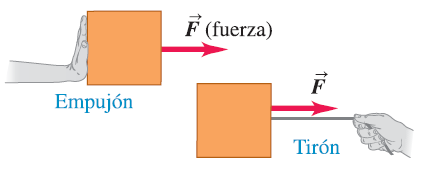
\includegraphics[scale=0.8]{Imagenes/Fuerza_01.png}
\end{figure}
\end{frame}
\begin{frame}
\frametitle{Definición}
Una \textocolor{byzantine}{fuerza} es una interacción entre dos cuerpos o entre un cuerpo y su ambiente.
\end{frame}
\begin{frame}
\frametitle{Fuerza como vector}
La fuerza es una cantidad vectorial, por lo que tiene una magnitud, dirección y sentido.
\end{frame}

\subsection{Tipos de fuerza}

\begin{frame}
\frametitle{Fuerza de contacto}
Una \textocolor{cobalt}{fuerza de contacto}, es aquella fuerza que implica un contacto directo entre dos cuerpos, como un empujón o un tirón.
\end{frame}
\begin{frame}
\frametitle{Tipos de fuerza de contacto}
\setbeamercolor{item projected}{bg=bananayellow,fg=ao}
\setbeamertemplate{enumerate items}{%
\usebeamercolor[bg]{item projected}%
\raisebox{1.5pt}{\colorbox{bg}{\color{fg}\footnotesize\insertenumlabel}}%
}
\begin{enumerate}[<+->]
\item Normal.
\item Fricción.
\item Tensión.
\end{enumerate}
\end{frame}
\begin{frame}
\frametitle{Fuerza normal}
Cuando un objeto descansa o se empuja sobre una superficie, ésta ejerce un empujón sobre el objeto que \textocolor{red}{es perpendicular} a la superficie.
\pause
\begin{figure}
    \centering
    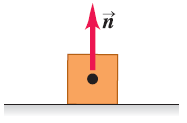
\includegraphics[scale=0.6]{Imagenes/Fuerza_02.png}
    \hspace*{1.5cm}
    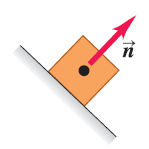
\includegraphics[scale=0.6]{Imagenes/Fuerza_03.png}
\end{figure}
\end{frame}
\begin{frame}
\frametitle{Fuerza de Fricción}
Se presenta cuando una superficie ejerce una fuerza que \textocolor{cerise}{es paralela} al objeto.
\begin{figure}
    \centering
    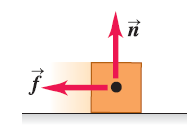
\includegraphics[scale=0.7]{Imagenes/Fuerza_04.png}
\end{figure}
\end{frame}
\begin{frame}
\frametitle{Fuerza de Tensión}
Es aquella fuerza \textocolor{cadmiumgreen}{de tirón} ejercida sobre un objeto por una cuerda, un cordón, etc.
\begin{figure}
    \centering
    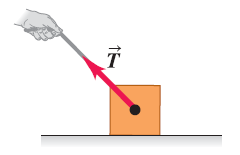
\includegraphics[scale=0.7]{Imagenes/Fuerza_05.png}
\end{figure}
\end{frame}
\begin{frame}
\frametitle{Fuerzas de largo alcance}
Son aquellas fuerzas que actúan aunque los cuerpos estén separados.
\pause
\begin{figure}
    \centering
    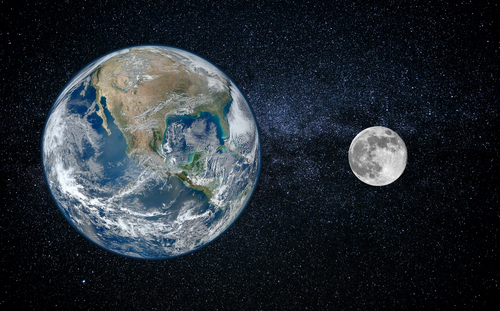
\includegraphics[scale=1.3]{Imagenes/Fuerza_09.jpg}
\end{figure}
\end{frame}

\subsection{Representación de una fuerza}

\begin{frame}
\frametitle{Representación de una fuerza}
Para describir una fuerza vectorial debemos indicar:
\setbeamercolor{item projected}{bg=aquamarine,fg=black}
\setbeamertemplate{enumerate items}{%
\usebeamercolor[bg]{item projected}%
\raisebox{1.5pt}{\colorbox{bg}{\color{fg}\footnotesize\insertenumlabel}}%
}
\begin{enumerate}[<+->]
\item Su dirección de acción.
\item Su magnitud, \pause es decir, la cantidad que describe \enquote{cuánto} o \enquote{qué tan tanto} la fuerza empuja o tira.
\end{enumerate}
\end{frame}
\begin{frame}
\frametitle{Unidad de la fuerza}
La unidad que mide la magnitud de fuerza en el Sistema Internacional, es el \textocolor{alizarin}{Newton}, que se abrevia \unit{\newton}.
\end{frame}
\begin{frame}
\frametitle{¿Qué representa un newton?}
El newton representa la unidad de fuerza necesaria para que un objeto de \textocolor{blue}{un kilogramo}, obtenga una aceleración de \textocolor{blue-violet}{un metro por segundo al cuadrado}:
\pause
\begin{align*}
\unit{\newton} \hspace{0.5cm} \Rightarrow \hspace{0.5cm} \left[ \unit[per-mode=fraction]{\kilo\gram\meter\per\square\second} \right]
\end{align*}
\end{frame}

\section{Suma de fuerzas}

\begin{frame}
\frametitle{Más de una fuerza actuando}
Los experimentos muestran que si dos fuerzas y actúan al mismo tiempo en un punto A de un cuerpo, \pause el efecto sobre el movimiento del cuerpo \textocolor{burgundy}{es igual al de una sola fuerza} igual a la suma vectorial de las fuerzas originales.
\end{frame}
\begin{frame}
\frametitle{Suma vectorial}
El resultado de la suma vectorial, es $\va{R}$, \pause es el \textocolor{cinnabar}{vector resultante}.
\pause
\begin{figure}
    \centering
    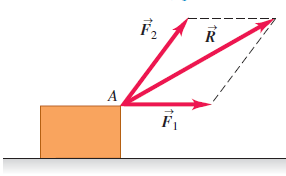
\includegraphics[scale=0.8]{Imagenes/Fuerza_06.png}
\end{figure}
\end{frame}
\begin{frame}
\frametitle{Para el caso con más fuerzas}
En general, el efecto de cualquier cantidad de fuerzas aplicadas a un punto de un cuerpo es el mismo de una sola fuerza igual a la suma vectorial de las fuerzas.
\end{frame}
\begin{frame}
\frametitle{Principio importante en física}
Éste es el importante \textocolor{coolblack}{principio de superposición de fuerzas}.
\end{frame}
\begin{frame}
\frametitle{Uso de un tema revisado}
Como la fuerza es un vector, podemos estudiarla a partir de las componentes vectoriales, \pause tal y como lo vimos en el tema de vectores.
\end{frame}
\begin{frame}
\frametitle{Componentes de una fuerza}
Para un vector que forma un ángulo con respecto a la horizontal, se tiene que:
\pause
\begin{figure}
    \centering
    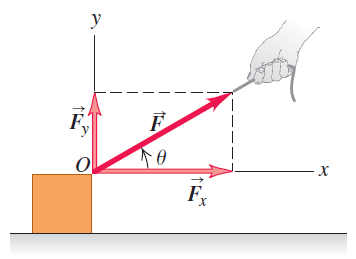
\includegraphics[scale=0.7]{Imagenes/Fuerza_07.png}
\end{figure}
\end{frame}
\begin{frame}
\frametitle{Componentes de una fuerza}
Las componentes $F_{x}$ y $F_{y}$ tienen juntas el mismo efecto que la fuerza original $\va{F}$.
\pause
\begin{figure}
    \centering
    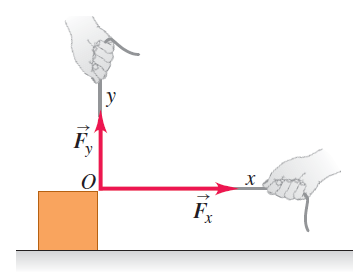
\includegraphics[scale=0.65]{Imagenes/Fuerza_08.png}
\end{figure}
\end{frame}
\begin{frame}
\frametitle{Un sistema de fuerzas}
Para resolver en una fuerza resultante, trabajamos con los vectores como lo hicimos en el tema anterior:
\pause
\setbeamercolor{item projected}{bg=red,fg=white}
\setbeamertemplate{enumerate items}{%
\usebeamercolor[bg]{item projected}%
\raisebox{1.5pt}{\colorbox{bg}{\color{fg}\footnotesize\insertenumlabel}}%
}
\begin{enumerate}[<+->]
\item Tabla de vectores por cuadrante, magnitud y ángulo.
\item Tabla de componentes por vector en el eje $x$ y en el eje $y$.
\seti
\end{enumerate}
\end{frame}
\begin{frame}
\frametitle{Un sistema de fuerzas}
\setbeamercolor{item projected}{bg=red,fg=white}
\setbeamertemplate{enumerate items}{%
\usebeamercolor[bg]{item projected}%
\raisebox{1.5pt}{\colorbox{bg}{\color{fg}\footnotesize\insertenumlabel}}%
}
\begin{enumerate}[<+->]    
\conti
\item Obtener la magnitud del vector resultante.
\item Obtener el ángulo del vector resultante.
\end{enumerate}
\end{frame}
\begin{frame}
\frametitle{Tabla de vectores}
\begin{table}
\centering
\begin{tabular}{c | c | c | c}
Vector & Cuadrante & Magnitud & Ángulo \\ \hline
$F_{1}$ & & & \\ \hline
$F_{2}$ & & & \\ \hline
$\ldots$ & & & \\ \hline 
\end{tabular}
\end{table}
\end{frame}
\begin{frame}
\frametitle{Tabla de componentes}
\begin{table}
\centering
\begin{tabular}{c | c | c | c}
Componente & Expresión & Sustitución & Valor \\ \hline
$F_{1x}$ & & & \\ \hline
$F_{1y}$ & & & \\ \hline    
$F_{2x}$ & & & \\ \hline
$F_{2y}$ & & & \\ \hline    
\end{tabular}
\end{table}
\end{frame}
\begin{frame}
\frametitle{Componentes de la resultante}
Las componentes $R_{x}$ y $R_{y}$ del vector resultante son:
\pause
\begin{eqnarray*}
\begin{aligned}
R_{x} = \nsum_{i=1}^{n} F_{ix} \\[0.5em] \pause
R_{y} = \nsum_{i=1}^{n} F_{iy}
\end{aligned}
\end{eqnarray*}
\end{frame}
\begin{frame}
\frametitle{Magnitud dl vector fuerza resultante}
La magnitud del vector fuerza resultantes es:
\pause
\begin{eqnarray*}
\begin{aligned}
\abs{\va{R}} = \pause \sqrt{(R_{x})^{2} + (R_{y})^{2}}
\end{aligned}
\end{eqnarray*}
\end{frame}
\begin{frame}
\frametitle{Ángulo del vector fuerza resultante}
El ángulo que determina la dirección del vector fuerza resultante es:
\pause
\begin{align*}
\theta_{R} = \tan^{-1} \left( \dfrac{R_{y}}{R_{x}} \right)
\end{align*}
\end{frame}

\section{Dinámica}
\frame{\tableofcontents[currentsection, hideothersubsections]}
\subsection{Introducción}

\begin{frame}
\frametitle{Preguntas disparadoras}
¿Cuáles son las causas del movimiento? 
\end{frame}
\begin{frame}
\frametitle{Preguntas disparadoras}
¿Cómo puede un remolcador empujar un trasatlántico que es mucho más pesado que él?
\pause
\begin{figure}
    \centering
    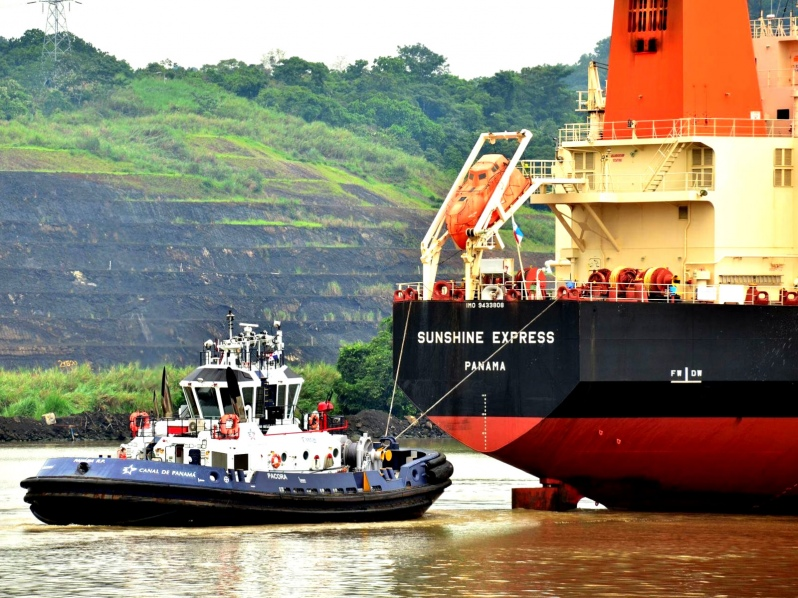
\includegraphics[scale=0.2]{Imagenes/Fuerza_10.jpg}
\end{figure}
\end{frame}
\begin{frame}
\frametitle{Preguntas disparadoras}
¿Por qué es más difícil controlar un automóvil en hielo mojado que en concreto seco?
\begin{figure}
    \centering
    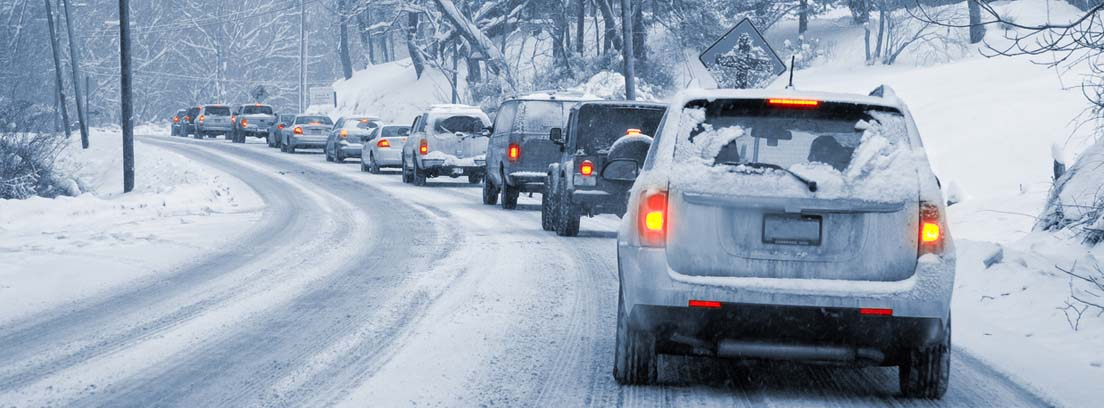
\includegraphics[scale=0.2]{Imagenes/Fuerza_11.jpg}
\end{figure}
\end{frame}
\begin{frame}
\frametitle{Respuestas a las Preguntas}
Las respuestas a estas preguntas y a otras similares nos llevan al tema de la \textocolor{coquelicot}{dinámica}, \pause es decir, la relación entre el movimiento y las fuerzas que lo causan.
\end{frame}
\begin{frame}
\frametitle{Conceptos necesarios}
Para apoyar nuestra revisión, utilizaremos los conceptos de \textocolor{cordovan}{fuerza} y la \textocolor{darkcyan}{masa}, para analizar los principios de la dinámica.
\end{frame}
\begin{frame}
\frametitle{Masa y peso}
Recordemos que:
\setbeamercolor{item projected}{bg=deepchampagne,fg=black}
\setbeamertemplate{enumerate items}{%
\usebeamercolor[bg]{item projected}%
\raisebox{1.5pt}{\colorbox{bg}{\color{fg}\footnotesize\insertenumlabel}}%
}
\begin{enumerate}[<+->]
\item Masa es la cantidad de sustancia que contiene un cuerpo, \pause en el sistema MKS su unidad es el \unit{\kilo\gram}, \pause en el sistema cgs, la unidad es el \unit{\gram}.
\seti
\end{enumerate}
\end{frame}
\begin{frame}
\frametitle{Masa y peso}
\setbeamercolor{item projected}{bg=deepchampagne,fg=black}
\setbeamertemplate{enumerate items}{%
\usebeamercolor[bg]{item projected}%
\raisebox{1.5pt}{\colorbox{bg}{\color{fg}\footnotesize\insertenumlabel}}%
}
\begin{enumerate}[<+->]
\conti
\item Peso es la masa multiplicada por el valor de \textbf{g}, \pause la aceleración debida a la gravedad: \SI{9.81}{\meter\per\square\second}, \pause las unidades del peso son los Newtons (\unit{\newton})
\pause
\begin{align*}
W = m \, g \hspace{0.5cm} \Rightarrow \hspace{0.5cm} \left[ \unit{\newton} \right]
\end{align*}
\end{enumerate}
\end{frame}    
\begin{frame}
\frametitle{Los primeros principios}
Estos principios se establecieron en sólo tres leyes que fueron claramente enunciadas por Sir Isaac Newton.
\begin{figure}
    \centering
    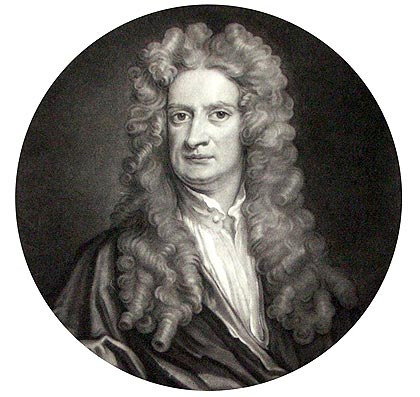
\includegraphics[scale=0.35]{Imagenes/Newton.jpg}
\end{figure}
\end{frame}

\section{Las leyes de Newton}
\frame{\tableofcontents[currentsection, hideothersubsections]}
\subsection{Primera ley}

\begin{frame}
\frametitle{Ley de la inercia}
Un cuerpo sobre el que no actúa una fuerza neta se mueve con velocidad constante (que puede ser cero) y aceleración cero.
\end{frame}
\begin{frame}
\frametitle{La ley de la inercia}
Un objeto en reposo permanece en reposo \pause y un objeto en movimiento, continuará en movimiento con una velocidad constante \pause a menos que se aplique una fuerza externa neta para modificar dicho estado.
\end{frame}
\begin{frame}
\frametitle{Ejemplo de la primera ley}
\begin{figure}
    \centering
    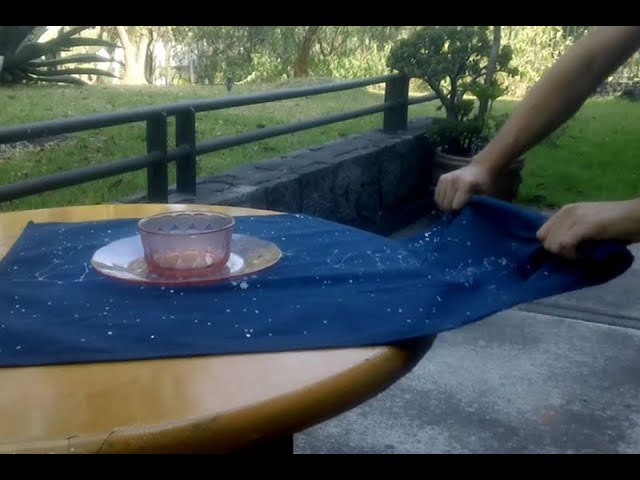
\includegraphics[scale=0.35]{Imagenes/Newton_01.jpg}
\end{figure}
\end{frame}
\begin{frame}
\frametitle{Concepto de inercia}
La tendencia de un cuerpo a seguir moviéndose una vez iniciado su movimiento es resultado de una propiedad llamada \textocolor{darkmagenta}{inercia}.
\end{frame}

\subsection{Segunda ley}

\begin{frame}
\frametitle{Fuerza sobre un cuerpo}
Si una \textocolor{darkscarlet}{fuerza externa neta} actúa sobre un cuerpo, éste se acelera.
\\
\bigskip
\pause
La dirección de aceleración es la misma que la dirección de la fuerza neta. 
\end{frame}
\begin{frame}
\frametitle{Expresión para la segunda ley}
El vector de fuerza neta es igual a la masa del cuerpo multiplicada por su aceleración.
\pause
\begin{align*}
\va{F} = m \, \va{a}
\end{align*}
\end{frame}
\begin{frame}
\frametitle{La segunda ley de Newton}
La segunda ley de Newton es una ley fundamental de la naturaleza, \pause \textocolor{darkslateblue}{la relación básica entre fuerza y movimiento}.
\end{frame}
\begin{frame}
\frametitle{El triángulo de la fuerza}
Ocupamos una referencia gráfica para el uso de la segunda ley de Newton: \pause \textocolor{debianred}{el triángulo de la fuerza}:
\pause
\begin{figure}
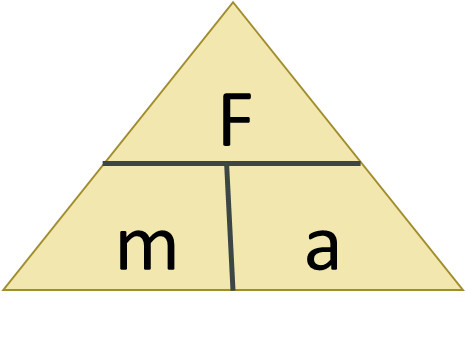
\includegraphics[scale=1]{Imagenes/Newton_11.jpg}
\end{figure}
\end{frame}
\begin{frame}
\frametitle{Ejercicio con la segunda ley}
Un trabajador aplica una fuerza horizontal constante con magnitud de \SI{20}{\newton} a una caja con masa de \SI{40}{\kilo\gram} que descansa en un piso plano con fricción despreciable.
\\
\bigskip
\pause
¿Qué aceleración experimenta la caja?.
\end{frame}
\begin{frame}
\frametitle{Entendiendo el ejercicio}
\begin{figure}
    \centering
    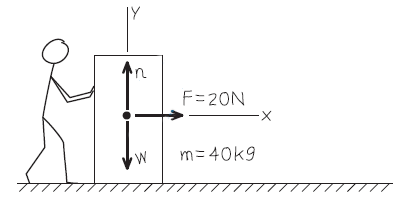
\includegraphics[scale=1]{Imagenes/Newton_02.png}
\end{figure}
\end{frame}
\begin{frame}
\frametitle{Resolviendo el ejercicio}
\textocolor{red}{Datos:}
\pause
\begin{align*}
F &= \SI{20}{\newton} \\[0.5em]
m &= \SI{40}{\kilo\gram}
\end{align*}
\end{frame}
\begin{frame}
\frametitle{Resolviendo el ejercicio}
\textocolor{red}{Expresión:}
\pause
\begin{figure}
    \centering
    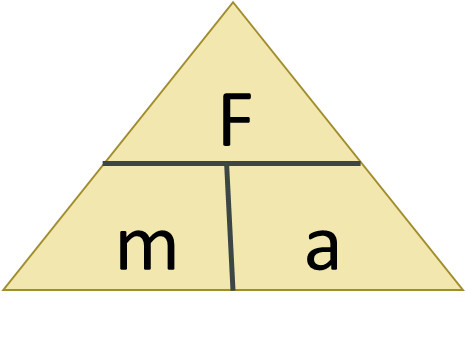
\includegraphics[scale=1]{Imagenes/Newton_11.jpg}
\end{figure}
\pause
\begin{align*}
a = \dfrac{F}{m}
\end{align*}
\end{frame}
\begin{frame}
\frametitle{Resolviendo el ejercicio}
\textocolor{red}{Sustitución:}
\pause
\begin{eqnarray*}
\begin{aligned}
a &= \dfrac{F}{m} = \pause \dfrac{\SI{20}{\newton}}{\SI{40}{\kilo\gram}} = \\[0.5em] \pause
a &= 0.5 \, \dfrac{\dfrac{\unit{\kilo\gram\meter}}{\unit{\square\second}}}{\unit{\kilo\gram}} = \\[0.5em] \pause 
a &= 0.5 \, \dfrac{\unit{\kilo\gram\meter}}{\unit{\kilo\gram\square\second}} = \pause \SI[per-mode=fraction]{0.5}{\meter\per\square\second}
\end{aligned}
\end{eqnarray*}
\end{frame}
\begin{frame}
\frametitle{Sobre las unidades}
Conviene aclarar que en el sistema \textbf{MKS}, \pause se utilizan las unidades de metro, kilogramo y segundo, como unidades de longitud, masa y tiempo, respectivamente.
\end{frame}
\begin{frame}
\frametitle{Sobre las unidades}
En ciencia e ingeniería se utiliza también un sistema llamado \textbf{cgs}, \pause donde las unidades de longitud, masa y tiempo son: el centímetro, gramo y segundo.
\end{frame}
\begin{frame}
\frametitle{Unidad de fuerza en cgs}
La unidad de medida de la fuerza en el sistema \textbf{cgs}, es la llamada \textocolor{denim}{dina}:
\pause
\begin{align*}
1 \, \text{dina} = \SI[per-mode=fraction]{1}{\gram\centi\meter\per\square\second}
\end{align*}
Sería conveniente que construyas el factor de conversión de dinas a Newtons.
\end{frame}
% \begin{frame}
% \frametitle{Unidad de fuerza sistema inglés}
% En el sistema británico, las unidades de:
% \pause
% \setbeamercolor{item projected}{bg=ferrarired,fg=white}
% \setbeamertemplate{enumerate items}{%
% \usebeamercolor[bg]{item projected}%
% \raisebox{1.5pt}{\colorbox{bg}{\color{fg}\footnotesize\insertenumlabel}}%
% }
% \begin{enumerate}[<+->]
% \item Fuerza es la \textocolor{ao}{libra} (o libra-fuerza).
% \item Masa es el \textocolor{electricindigo}{slug}.
% \item Aceleración es el pie por segundo al cuadrado.
% \end{enumerate}
% \end{frame}
% \begin{frame}
% \frametitle{Unidad de fuerza sistema inglés}
% Así que la unidad de fuerza en el sistema inglés es:
% \pause
% \begin{align*}
% 1 \, \text{libra-fuerza} = \text{slug} \, \dfrac{\text{pie}}{\unit{\square\second}}
% \end{align*}
% \end{frame}
\begin{frame}
\frametitle{Enunciado de otro ejercicio}
Determina la fuerza que se necesita aplicar a un auto de \SI{800}{\kilo\gram} para que éste se acelere \SI{4}{\meter\per\square\second}.
\end{frame}
\begin{frame}
\frametitle{Resolviendo el ejercicio}
\textocolor{red}{Datos:}
\pause
\begin{align*}
m &= \SI{800}{\kilo\gram} \\[0.5em]
a &= \SI{4}{\meter\per\square\second} \\[0.5em]
F &= \, ?
\end{align*}
\end{frame}
\begin{frame}
\frametitle{Resolviendo el ejercicio}
\textocolor{red}{Expresión:}
\pause
\begin{figure}
    \centering
    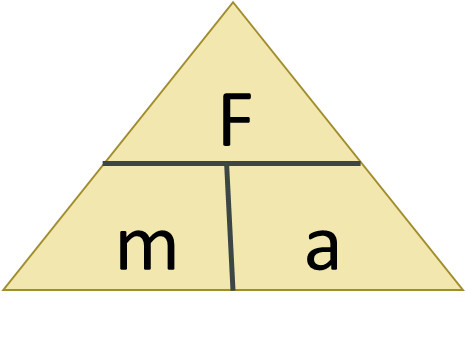
\includegraphics[scale=1]{Imagenes/Newton_11.jpg}
\end{figure}
\pause
\begin{align*}
F = m \, a
\end{align*}
\end{frame}
\begin{frame}
\frametitle{Resolviendo el ejercicio}
\textocolor{red}{Sustitución:}
\pause
\begin{eqnarray*}
\begin{aligned}
F &= \left( \SI{800}{\kilo\gram} \right) \left( \SI{4}{\meter\per\square\second} \right) = \\[0.5em] \pause
F &= \SI[per-mode=fraction]{3.2d3}{\kilo\gram\meter\per\square\second} = \pause \SI{3.2d3}{\newton}
\end{aligned}
\end{eqnarray*}
\end{frame}    
\begin{frame}
\frametitle{Enunciado de otro ejercicio}
El resultado de las fuerzas que actúan sobre un cuerpo cuya masa vale \SI{40}{\kilo\gram}, es de \SI{85}{\newton}
\\
\bigskip
¿Cuál es el valor de la aceleración que posee este cuerpo?
\end{frame}
\begin{frame}
\frametitle{Resolviendo el ejercicio}
\textocolor{red}{Datos:}
\pause
\begin{align*}
m &= \SI{40}{\kilo\gram} \\[0.5em]
F &= \SI{85}{\newton} \\[0.5em]
a &= \, ?
\end{align*}
\end{frame}
\begin{frame}
\frametitle{Resolviendo el ejercicio}
\textocolor{red}{Expresión:}
\pause
\begin{figure}
    \centering
    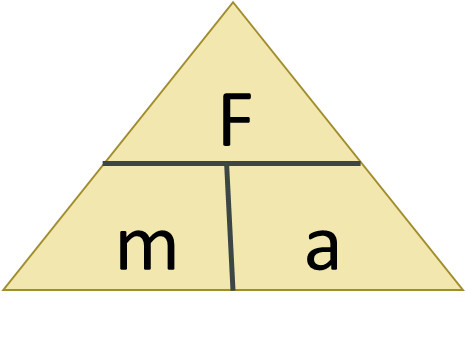
\includegraphics[scale=1]{Imagenes/Newton_11.jpg}
\end{figure}
\pause
\begin{align*}
a = \dfrac{F}{m}
\end{align*}
\end{frame}
\begin{frame}
\frametitle{Resolviendo el ejercicio}
\textocolor{red}{Sustitución:}
\pause
\begin{eqnarray*}
\begin{aligned}
a &= \dfrac{\SI{85}{\newton}}{\SI{40}{\kilo\gram}} = \\[0.5em] \pause
a &= 2.125 \, \dfrac{\dfrac{\unit{\kilo\gram\meter}}{\unit{\square\second}}}{\unit{\kilo\gram}} = \pause 2.125 \, \dfrac{\unit{\kilo\gram\meter}}{\unit{\kilo\gram\square\second}} \\[0.5em] \pause
a &= \SI[per-mode=fraction]{2.125}{\meter\per\square\second}
\end{aligned}
\end{eqnarray*}
\end{frame}
\begin{frame}
\frametitle{Ejercicio más elaborado}
¿Qué fuerza debe ejercer el motor de un automóvil cuya masa es de \SI{1500}{\kilo\gram} para aumentar su velocidad de \SI{4.5}{\kilo\meter\per\hour} a \SI{40}{\kilo\meter\per\hour} en \SI{8}{\second}?
\end{frame}
\begin{frame}
\frametitle{Resolviendo el ejercicio más elaborado}
\textocolor{red}{Datos:}
\pause
\begin{eqnarray*}
\begin{aligned}
m &= \SI{1500}{\kilo\gram} \\[0.25em] \pause
F &= \, ? \\[0.25em] \pause
a &= \, ? \\[0.25em] \pause
v_{i} &= \SI{4.5}{\kilo\meter\per\hour} \\[0.25em] \pause
v_{f} &= \SI{40}{\kilo\meter\per\hour}
\end{aligned}
\end{eqnarray*}
\end{frame}
\begin{frame}
\frametitle{Resolviendo el ejercicio más elaborado}
\textocolor{red}{Expresión:}
\\
\begin{minipage}{0.4\linewidth}
\begin{figure}
    \centering
    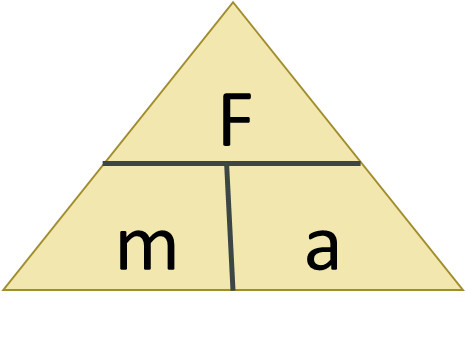
\includegraphics[scale=0.75]{Imagenes/Newton_11.jpg}
\end{figure}
\end{minipage}
\begin{minipage}{0.4\linewidth}
\begin{align*}
F = m \, a
\end{align*}
\end{minipage}
\pause
\begin{align*}
a = \dfrac{v_{f} - v_{i}}{t}
\end{align*}
\end{frame}
\begin{frame}
\frametitle{Ajustando las unidades}
El valor de la velocidad se indica en \unit{\kilo\meter\per\hour}, el tiempo en el que hay un cambio de velocidad, es decir, la aceleración, se da en segundos, por lo que hay que ajustar las unidades y manejar las mismas.
\end{frame}
\begin{frame}
\frametitle{Conversión de unidades}
\begin{eqnarray*}
\begin{aligned}
v_{i} &= \SI[per-mode=fraction]{4.5}{\kilo\meter\per\hour} \left( \dfrac{\SI{1d3}{\meter}}{\SI{1}{\kilo\meter}} \right) \left( \dfrac{\SI{1}{\hour}}{\SI{3600}{\second}} \right) = \pause \SI[per-mode=fraction]{1.25}{\meter\per\second} \\[0.5em] \pause
v_{f} &= \SI[per-mode=fraction]{40}{\kilo\meter\per\hour} \left( \dfrac{\SI{1d3}{\meter}}{\SI{1}{\kilo\meter}} \right) \left( \dfrac{\SI{1}{\hour}}{\SI{3600}{\second}} \right) = \pause \SI[per-mode=fraction]{11.11}{\meter\per\second} \\[0.5em] \pause
\end{aligned}
\end{eqnarray*}
\end{frame}
\begin{frame}
\frametitle{Resolviendo el ejercicio}
\textocolor{red}{Sustitución. } Para la aceleración:
\pause
\begin{eqnarray*}
\begin{aligned}
a &= \dfrac{ \displaystyle \SI[per-mode=fraction]{11.11}{\meter\per\second} - \SI[per-mode=fraction]{1.25}{\meter\per\second}}{\SI{8}{\second}} = \pause \dfrac{\displaystyle \SI[per-mode=fraction]{9.86}{\meter\per\second}}{\SI{8}{\second}} = \\[0.5em] \pause
a &= \SI[per-mode=fraction]{1.23}{\meter\per\square\second}
\end{aligned}
\end{eqnarray*}  
\end{frame}
\begin{frame}
\frametitle{Resolviendo el ejercicio}
\textocolor{red}{Sustitución. } Para la fuerza:
\pause
\begin{eqnarray*}
\begin{aligned}
F &= \left( \SI{1500}{\kilo\gram} \right) \left( \SI[per-mode=fraction]{1.23}{\meter\per\square\second} \right) \\[0.5em] \pause
F &= \SI[per-mode=fraction]{1845}{\kilo\gram\meter\per\square\second} = \pause \SI{1845}{\newton}
\end{aligned}
\end{eqnarray*}  
\end{frame}

% \subsection{Tercera ley}

% \begin{frame}
% \frametitle{La tercera ley de Newton}
% La tercera Ley de Newton indica que cuando \textocolor{denim}{un cuerpo ejerce una fuerza sobre otro}, \pause \textocolor{red}{el segundo ejerce siempre sobre el primero una fuerza de igual magnitud pero de sentido opuesto}.
% \end{frame}
% \begin{frame}
% \frametitle{La tercera ley de Newton}
% A la tercera ley de Newton, se le conoce como \pause \textocolor{auburn}{ley de acción y reacción}.
% \\
% \bigskip
% \pause
% A cada fuerza de acción, le corresponde una fuerza de reacción.
% \end{frame}
% \begin{frame}
% \frametitle{Ejemplo de la tercera ley de Newton}
% \begin{figure}
%     \centering
%     \only<1>{
\includegraphics[scale=3]{Imagenes/Pateando_Balon_01.png}}
%     \only<2>{
\includegraphics[scale=3]{Imagenes/Pateando_Balon_02.png}}
% \end{figure}
% \end{frame}
% \begin{frame}
% \frametitle{Resumen}
% Las tres leyes de Newton son:
% \pause
% \setbeamercolor{item projected}{bg=bananayellow,fg=black}
% \setbeamertemplate{enumerate items}{%
% \usebeamercolor[bg]{item projected}%
% \raisebox{1.5pt}{\colorbox{bg}{\color{fg}\footnotesize\insertenumlabel}}%
% }
% \begin{enumerate}[<+->]
% \item Ley de la inercia.
% \item Ley de la relación entre la fuerza y la aceleración.
% \item Ley de la acción y reacción.
% \end{enumerate}
% \end{frame}

% \subsection{Fuerza normal}

% \begin{frame}
% \frametitle{La fuerza normal}
% Si se considera un objeto en reposo $(v = 0)$ sobre una superficie horizontal, \pause sabemos que el centro de la Tierra ejerce sobre él la fuerza gravitacional, \pause a pesar de no tener aceleración $(a = 0)$.
% \begin{figure}
%     \centering
%     \begin{tikzpicture}
%         \draw (0, 0) -- (3, 0);
%         \draw (1, 0) rectangle (2, 0.5) node [pos=0.5] {\small{$m$}};
%         \draw [-stealth, thick] (1.5, 0) -- (1.5, -1);
%         \node at (1.3, -1.4) {\small{$W = m \, g$}};
%     \end{tikzpicture}
% \end{figure}
% \end{frame}
% \begin{frame}
% \frametitle{La fuerza normal}
% De acuerdo con la segunda ley de Newton, \pause \textocolor{red}{la fuerza neta} que actúa sobre el objeto \textocolor{red}{es cero}, \pause por lo tanto, debe existir una fuerza que se oponga a la fuerza gravitacional y que actúe sobre el objeto para impedir que éste se hunda.
% \end{frame}
% \begin{frame}
% \frametitle{La fuerza normal}
% Esta fuerza es producida por la superficie, actúa de manera perpendicular a la superficie de contacto, se llama \textocolor{cobalt}{fuerza normal} $F_{n}$.
% \pause
% \begin{figure}
%     \centering
%     \begin{tikzpicture}
%         \draw (0, 0) -- (3, 0);
%         \draw (1, 0) rectangle (2, 0.5) node [pos=0.5] {\small{$m$}};
%         \draw [-stealth, thick] (1.5, 0) -- (1.5, -1);
%         \node at (1.3, -1.4) {\small{$W = m \, g$}};

%         \draw (5, 0) -- (6, 0);
%         \draw [-stealth, thick] (5.5, 0) -- (5.5, -1);
%         \node at (5.5, -1.4) {\small{$W = m \, g$}};
%         \draw [-stealth, thick] (5.5, 0) -- (5.5, 1);
%         \node at (5.5, 1.4) {\small{$F_{n}$}};
%     \end{tikzpicture}
% \end{figure}
% \end{frame}
% \begin{frame}
% \frametitle{Magnitud de la fuerza normal}
% Por la segunda ley de Newton:
% \pause
% \begin{eqnarray*}
% \begin{aligned}
% \nsum F_{y} &= 0 \\[0.5em] \pause
% F_{n} -  m \, g &= 0 \\[0.5em] \pause
% F_{n} &=  m \, g 
% \end{aligned}
% \end{eqnarray*}
% \end{frame}

% \subsection{Plano inclinado}

% \begin{frame}
% \frametitle{El plano inclinado}
% Si un objeto descansa sobre un plano inclinado, actúan sobre él la fuerza gravitacional (el peso) y la fuerza normal $F_{n}$:
% \pause
% \begin{figure}
%     \centering
%     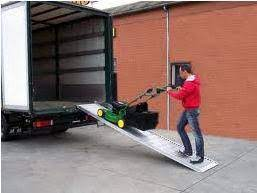
\includegraphics[scale=0.5]{Imagenes/Plano_inclinado_01.jpg}
% \end{figure}
% \end{frame}
% \begin{frame}
% \frametitle{Representación gráfica}
% Tendremos que el plano inclinado se visualiza:
% \pause
% \begin{figure}
% \centering
% \begin{tikzpicture}[scale=2]
%     \begin{scope}[rotate=15]
%         \draw (0, 0) -- (3, 0);
%         \draw (1, 0) rectangle (2, 0.5);
%         \draw [fill] (1.5, 0.25) circle (0.5pt);
%         \draw [-stealth, thick] (1.5, 0.25) -- (1.5, 1) node [near end, pos=1.2] {\small{$N$}};
%         \draw [dashed] (1.5, 0.25) -- (1.5, -1);
%         \draw [-stealth, thick] (1.5, 0.25) -- (1.25, -0.72) node [near end, pos=1.2] {\small{$W$}};
%     \end{scope}

%     \draw (0, 0) -- (1, 0);
%     \draw (0.5, 0) arc(0:15:0.5);
%     \node at (0.8, 0.1) {\small{$\theta$}};
% \end{tikzpicture}
% \end{figure}
% \end{frame}
% \begin{frame}
% \frametitle{Descomponiendo el peso}
% Si establecemos un sistema de coordenadas donde el eje $x$ es paralelo al plano inclinado, \pause mientras que el eje $y$ perpendicular al mismo, \pause se puede descomponer el vector peso $\vb{W}$ en sus componentes rectangulares $W_{x}$ y $W_{y}$:
% \end{frame}
% \begin{frame}
% \frametitle{Diagrama de cuerpo libre}
% \begin{figure}
% \centering
% \begin{tikzpicture}[scale=2]
%     \begin{scope}[rotate=15]
%         \draw (0, 0) -- (3, 0);
%         \draw [-stealth, thick] (1.5, 0) -- (1.5, 0.75) node [near end, pos=1.2] {\small{$N$}};
%         \draw [dashed] (1.5, 0.25) -- (1.5, -1);
%         \draw [-stealth, thick] (1.5, 0) -- (1.3, -0.75) node [near end, pos=1.2] {\small{$W$}};
%         \draw [-stealth] (1.5, 0) -- (1.3, 0) node [above, pos=1.1] {\footnotesize{$W_{x}$}};
%         \draw [-stealth] (1.5, 0) -- (1.5, -0.75) node [right, pos=1.1] {\footnotesize{$W_{y}$}};
%         \draw [dashed] (1.3, 0) -- (1.3, -0.75);
%         \draw [dashed] (1.5, -0.75) -- (1.3, -0.75);

%         \draw (1.5, -0.5) arc(270:255:0.5);
%         \node at (1.6, -0.5) {\footnotesize{$\theta$}};
%     \end{scope}

%     \draw (0, 0) -- (1, 0);
%     \draw (0.5, 0) arc(0:15:0.5);
%     \node at (0.8, 0.1) {\small{$\theta$}};
%     \pause
%     \node at (3.5, 1) {\small{Por geometría:}};
%     \node at (3.5, 0.6) {\small{$\cos \theta = \dfrac{W_{y}}{W}$}};
% \end{tikzpicture}
% \end{figure}
% \end{frame}
% \begin{frame}
% \frametitle{Revisando las expresiones}
% Por geometría, tenemos que:
% \pause
% \begin{eqnarray*}
% \begin{aligned}
% \cos \theta = \dfrac{W_{y}}{W} \pause \hspace{1cm} \Rightarrow \hspace{1cm} W_{y} = W \, \cos \theta
% \end{aligned}
% \end{eqnarray*}
% \end{frame}
% \begin{frame}
% \frametitle{Revisando las expresiones}    
% Como sabemos:
% \pause
% \begin{eqnarray*}
% \begin{aligned}
% W = m \, g  \pause \hspace{1cm} \Rightarrow \hspace{1cm} W_{y} = m \, g \, cos \theta
% \end{aligned}
% \end{eqnarray*}
% \end{frame}
% \begin{frame}
% \frametitle{Revisando las expresiones}
% De la misma manera:
% \pause
% \begin{eqnarray*}
% \begin{aligned}
% \sin \theta = \dfrac{W_{x}}{W} \pause \hspace{1cm} \Rightarrow \hspace{1cm} W_{x} = W \, sin \theta
% \end{aligned}
% \end{eqnarray*}
% \end{frame}
% \begin{frame}
% \frametitle{Fuerza normal}
% Para la fuerza normal: 
% \pause
% \begin{align*}
% \nsum F_{y} = m \, a_{y}
% \end{align*}
% \pause
% Como no hay movimiento:
% \pause
% \begin{eqnarray*}
% \begin{aligned}
% a_{y} = 0 \pause \hspace{0.5cm} \Rightarrow \hspace{0.5cm} N - W_{y} = 0 \pause \hspace{0.5cm} \Rightarrow \hspace{0.5cm} N = W_{y}
% \end{aligned}
% \end{eqnarray*}
% \pause
% Con lo que resulta $N = m \, g \, cos \theta$
% \end{frame}

% \section{La fricción}
% \frame{\tableofcontents[currentsection, hideothersubsections]}
% \subsection{Definiendo la fricción}

% \begin{frame}
% \frametitle{Entendiendo la fricción}
% Si se golpea una bola de billar sobre la mesa, su velocidad disminuye hasta que se detiene.
% \begin{figure}
%     \centering
%     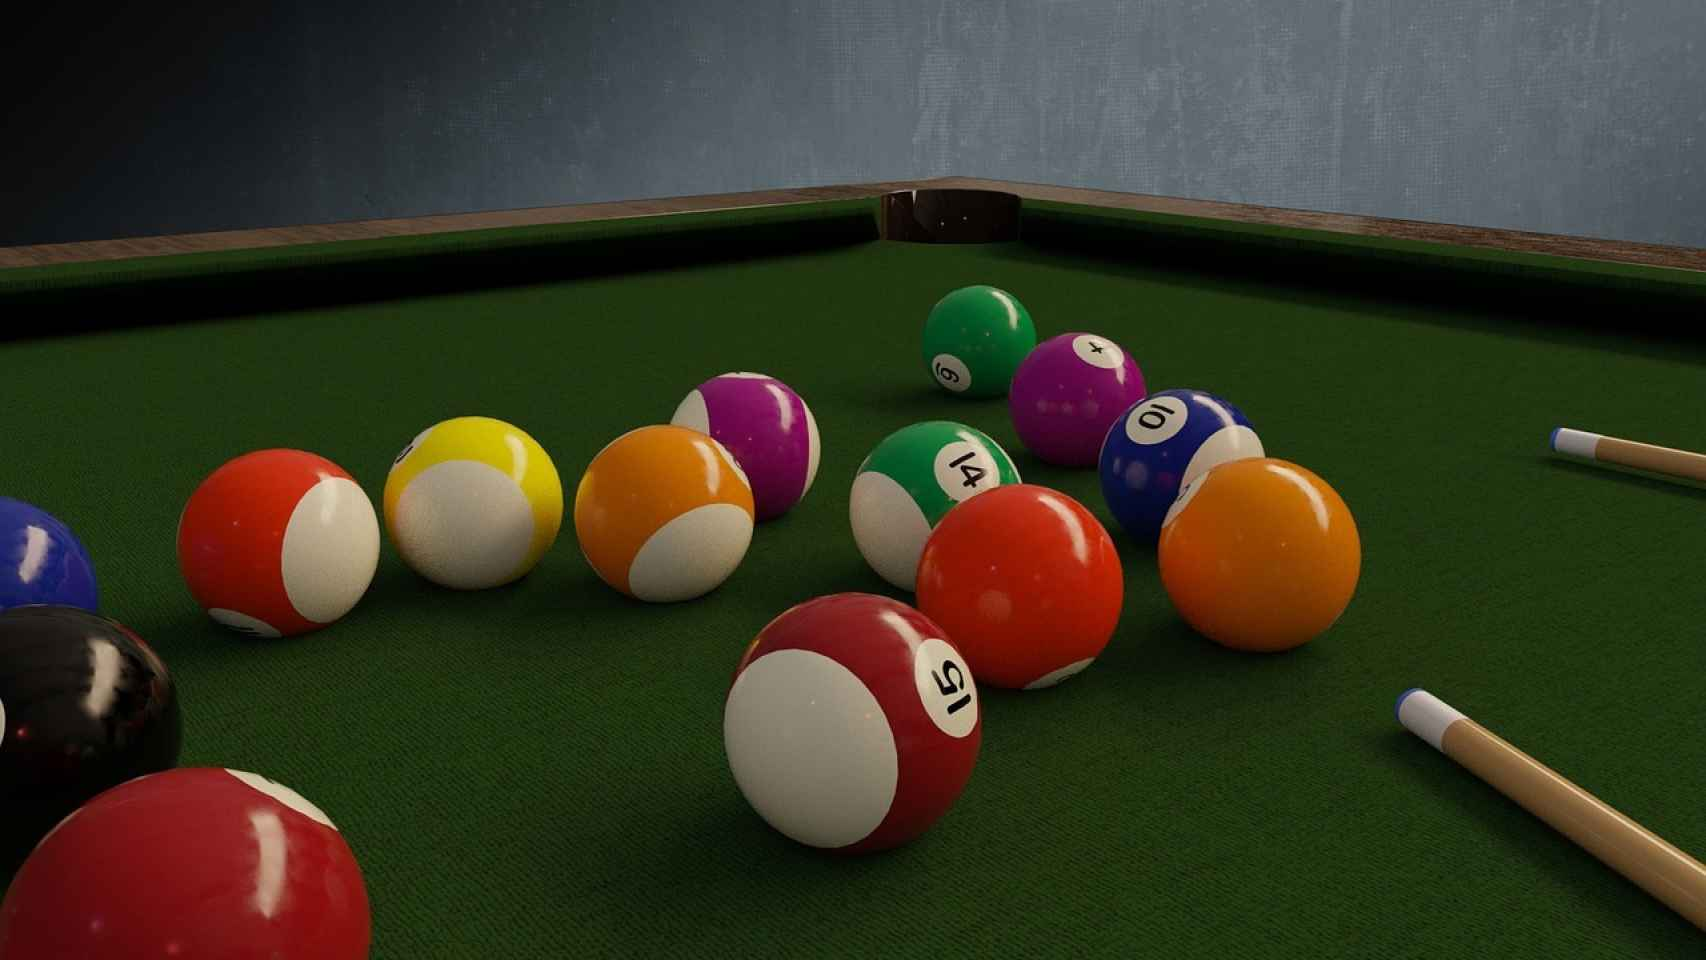
\includegraphics[scale=0.15]{Imagenes/Friccion_01.jpg}
% \end{figure}
% \end{frame}
% \begin{frame}
% \frametitle{Entendiendo la fricción}
% Esta desaceleración, de acuerdo con la \textocolor{burgundy}{primera ley de Newton}, \pause indica la \textocolor{byzantium}{existencia de una fuerza} que se opone al movimiento.
% \\
% \bigskip
% \pause
% Esta fuerza recibe el nombre de \textocolor{red}{fricción o rozamiento}.
% \end{frame}

% \subsection{Tipos de fricción}

% \begin{frame}
% \frametitle{Tipos de fricción}
% Existen dos tipos de fricciones:
% \pause
% \setbeamercolor{item projected}{bg=aquamarine,fg=black}
% \setbeamertemplate{enumerate items}{%
% \usebeamercolor[bg]{item projected}%
% \raisebox{1.5pt}{\colorbox{bg}{\color{fg}\footnotesize\insertenumlabel}}%
% }
% \begin{enumerate}[<+->]
% \item \textocolor{armygreen}{Fricción estática}: se presenta cuanto la fricción impide que un objeto se ponga en movimiento por la acción de una fuerza.
% \item \textocolor{arsenic}{Fricción cinética}: se presenta cuando la fricción se opone a un movimiento en acción.
% \end{enumerate}
% \end{frame}
% \begin{frame}
% \frametitle{Leyes de la fricción}
% \setbeamercolor{item projected}{bg=babypink,fg=black}
% \setbeamertemplate{enumerate items}{%
% \usebeamercolor[bg]{item projected}%
% \raisebox{1.5pt}{\colorbox{bg}{\color{fg}\footnotesize\insertenumlabel}}%
% }
% \begin{enumerate}[<+->]
% \item Para superficies paralelas, la fuerza de fricción estática ($f_{s}$) actúa en la dirección de la fuerza aplicada, en sentido contrario.
% \seti
% \end{enumerate}
% \end{frame}
% \begin{frame}
% \frametitle{Leyes de la fricción}
% \setbeamercolor{item projected}{bg=babypink,fg=black}
% \setbeamertemplate{enumerate items}{%
% \usebeamercolor[bg]{item projected}%
% \raisebox{1.5pt}{\colorbox{bg}{\color{fg}\footnotesize\insertenumlabel}}%
% }
% \begin{enumerate}[<+->]
% \conti
% \item La magnitud de la fuerza de fricción estática es directamente proporcional a la magnitud de la fuerza normal, y se calcula multiplicando el coeficiente de fricción estático ($\mu_{s}$) por la normal:
% \begin{align*}
% f_{s} = \mu_{s} \, N
% \end{align*}
% \seti
% \end{enumerate}
% \end{frame}
% \begin{frame}
% \frametitle{Leyes de la fricción}
% \setbeamercolor{item projected}{bg=babypink,fg=black}
% \setbeamertemplate{enumerate items}{%
% \usebeamercolor[bg]{item projected}%
% \raisebox{1.5pt}{\colorbox{bg}{\color{fg}\footnotesize\insertenumlabel}}%
% }
% \begin{enumerate}[<+->]
% \conti
% \item La magnitud de la fuerza de fricción estática es cero cuando no se aplica una fuerza externa que ponga el objeto en movimiento.
% \seti
% \end{enumerate}
% \end{frame}
% \begin{frame}
% \frametitle{Leyes de la fricción}
% \setbeamercolor{item projected}{bg=babypink,fg=black}
% \setbeamertemplate{enumerate items}{%
% \usebeamercolor[bg]{item projected}%
% \raisebox{1.5pt}{\colorbox{bg}{\color{fg}\footnotesize\insertenumlabel}}%
% }
% \begin{enumerate}[<+->]
% \conti
% \item La magnitud de la fuerza de fricción estática alcanza su punto máximo cuando un objeto está a punto de iniciar su movimiento mediante la acción de una fuerza paralela a las superficies que están en contacto.
% \seti
% \end{enumerate}
% \end{frame}
% \begin{frame}
% \frametitle{Leyes de la fricción}
% \setbeamercolor{item projected}{bg=babypink,fg=black}
% \setbeamertemplate{enumerate items}{%
% \usebeamercolor[bg]{item projected}%
% \raisebox{1.5pt}{\colorbox{bg}{\color{fg}\footnotesize\insertenumlabel}}%
% }
% \begin{enumerate}[<+->]
% \conti
% \item La fuerza de fricción cinética es directamente proporcional a la magnitud de la fuerza normal, y se calcula multiplicando el coeficiente de fricción cinético ($\mu_{k}$) por la normal
% \begin{align*}
% f_{k} = \mu_{k} \, N
% \end{align*}
% \seti
% \end{enumerate}
% \end{frame}
% \begin{frame}
% \frametitle{Leyes de la fricción}
% \setbeamercolor{item projected}{bg=babypink,fg=black}
% \setbeamertemplate{enumerate items}{%
% \usebeamercolor[bg]{item projected}%
% \raisebox{1.5pt}{\colorbox{bg}{\color{fg}\footnotesize\insertenumlabel}}%
% }
% \begin{enumerate}[<+->]
% \conti
% \item Se pueden presentar 3 casos cuando un objeto se desliza sobre una superficie y se le aplica una fuerza $F$ paralela a la superficie:
% \seti
% \end{enumerate}
% \end{frame}
% \begin{frame}
% \frametitle{Leyes de la fricción}
% 1. Si $F = f_{k}$ el objeto se desliza a velocidad constante. \\[0.25em] \pause
% 2. Si $F > f_{k}$ el objeto se acelera. \\[0.25em] \pause
% 3. Si $F < f_{k}$ el objeto se desacelera hasta detenerse por completo.
% \end{frame}
% \begin{frame}
% \frametitle{Leyes de la fricción}
% \setbeamercolor{item projected}{bg=babypink,fg=black}
% \setbeamertemplate{enumerate items}{%
% \usebeamercolor[bg]{item projected}%
% \raisebox{1.5pt}{\colorbox{bg}{\color{fg}\footnotesize\insertenumlabel}}%
% }
% \begin{enumerate}[<+->]
% \conti
% \item Si se deja aplicar la fuerza, la fuerza de fricción cinética desacelera el objeto hasta llevarlo al reposo.
% \item El coeficiente de fricción estática es mayor que el coeficiente de fricción cinética, es decir, $f_{s} > f_{k}$
% \end{enumerate}
% \end{frame}
% \begin{frame}
% \frametitle{Enunciado del ejercicio}
% Una señora desea mover un mueble hacia la izquierda. \pause El mueble pesa \SI{35}{\kilo\gram} y el coeficiente de fricción cinética $\mu_{k}$ entre ella y el suelo es $0.36$.
% \\
% \bigskip
% \pause
% Calcula la fuerza que debe emplear la señora para comenzar a mover el mueble.
% \end{frame}
% \begin{frame}
% \frametitle{Resolviendo el ejercicio}
% \textocolor{red}{Datos:}
% \pause
% \begin{align*}
% m &= \SI{35}{\kilo\gram} \\[0.2em]
% \mu_{k} &= \num{0.36} \\[0.2em]
% g &= \SI{9.81}{\meter\per\square\second} \\[0.2em]
% F &= \, ?
% \end{align*}
% \end{frame}
% \begin{frame}
% \frametitle{Resolviendo el ejercicio}
% \textocolor{red}{Expresiones:}
% \pause
% \begin{eqnarray*}
% \begin{aligned}
% N &= m \, g \\[0.3em]
% f_{k} &= \mu_{k} \, N
% \end{aligned}
% \end{eqnarray*}
% \end{frame}
% \begin{frame}
% \frametitle{Resolviendo el ejercicio}
% \textocolor{red}{Sustitución:}
% \begin{eqnarray*}
% \begin{aligned}
% N &= (\SI{35}{\kilo\gram})(\SI{9.81}{\meter\per\square\second}) = \pause \SI{343.35}{\newton} \\[0.5em] \pause
% f_{k} &= (0.36)(\SI{343.35}{\newton}) = \pause \SI{123.61}{\newton}
% \end{aligned}
% \end{eqnarray*}
% \end{frame}
% \begin{frame}
% \frametitle{Enunciado de otro ejercicio}
% Una caja de \SI{70}{\kilo\gram} que se desliza sobre una superficie horizontal es jalada por un hombre con una fuerza de \SI{140}{\newton} con un ángulo de \ang{40} con la horizontal.
% \\
% \bigskip
% \pause
% Calcula la aceleración del objeto si el coeficiente de fricción cinética es de \num{0.15}
% \end{frame}
% \begin{frame}
% \frametitle{Resolviendo el ejercicio}
% \textocolor{red}{Datos:}
% \pause
% \begin{minipage}[t]{0.4\linewidth}
% \begin{align*}
% m &= \SI{70}{\kilo\gram} \\[0.2em]
% \mu_{k} &= \num{0.15} \\[0.2em]
% g &= \SI{9.81}{\meter\per\square\second} \\[0.2em]
% \end{align*}
% \end{minipage}
% \begin{minipage}[t]{0.4\linewidth}
% \begin{align*}
% F &= \SI{140}{\newton} \\[0.2em]
% \theta &= \ang{40}\\[0.2em]
% a &= \, ?
% \end{align*}
% \end{minipage}
% \end{frame}
% \begin{frame}
% \frametitle{Resolviendo el ejercicio}
% \textocolor{red}{Expresiones:}
% \pause
% \begin{eqnarray*}
% \begin{aligned}
% F_{y} &= F \sin \theta \\[0.3em]
% F_{x} &= F \cos \theta \\[0.3em]
% N &= m \, g \\[0.3em]
% f_{k} &= \mu_{k} \, N
% \end{aligned}
% \end{eqnarray*}
% \end{frame}
% \begin{frame}
% \frametitle{Resolviendo el ejercicio}
% Para el eje $y$:
% \pause
% \begin{eqnarray*}
% \begin{aligned}
% N + F_{y} - W &= 0 \\[0.3em] \pause
% N &= W - F_{y} \\[0.3em] \pause
% N &= m \, g - F \, \sin \theta
% \end{aligned}
% \end{eqnarray*}
% \end{frame}
% \begin{frame}
% \frametitle{Resolviendo el ejercicio}
% \textocolor{red}{Sustitución:}
% \pause
% \begin{eqnarray*}
% \begin{aligned}
% N &= (\SI{70}{\kilo\gram})(\SI{9.81}{\meter\per\square\second}) - (\SI{140}{\newton})(\sin \ang{40}) = \\[0.5em] \pause
% N &= \SI{596.70}{\newton}
% \end{aligned}
% \end{eqnarray*}
% \end{frame}
% \begin{frame}
% \frametitle{Resolviendo el ejercicio}
% Para el eje $x$:
% \pause
% \begin{eqnarray*}
% \begin{aligned}
% F_{x} - f_{k} &= m \, a \\[0.3em] \pause
% a &= \dfrac{F_{x} - f_{k}}{m} = \pause \dfrac{F \, \cos \ang{40} - \mu_{k} \, N}{m} = \\[0.3em] \pause
% a &= \dfrac{(\SI{140}{\newton})(0.766) - (0.15)(\SI{596.70}{\newton})}{\SI{70}{\kilo\gram}} = \\[0.5em]\pause
% a &= \SI{0.25}{\meter\per\square\second}
% \end{aligned}
% \end{eqnarray*}
% \end{frame}

\section{Ley de gravitación universal}
\frame[allowframebreaks]{\tableofcontents[currentsection, hideothersubsections]}
\subsection{Definición}

\begin{frame}
\frametitle{La ley de gravitación universal}
La ley de la gravitación universal nos menciona de que toda partícula en el universo \textocolor{ao}{atrae a otra partícula con una fuerza} que:
\pause
\begin{quote}
“es directamente proporcional al producto de sus masas e inversamente proporcional al cuadrado de la distancia entre ellas”.
\end{quote}
\end{frame}
\begin{frame}
\frametitle{La expresión}
\vspace*{-1cm}
La ley de gravitación universal se expresa como:
\pause
\begin{align*}
F = G \, \dfrac{m_{1} \, m_{2}}{r^{2}}
\end{align*}
Donde:
\pause
\setbeamercolor{item projected}{bg=celadon,fg=black}
\setbeamertemplate{enumerate items}{%
\usebeamercolor[bg]{item projected}%
\raisebox{1.5pt}{\colorbox{bg}{\color{fg}\footnotesize\insertenumlabel}}%
}
\begin{enumerate}[<+->]
\item $F$ es la fuerza de atracción gravitacional.
\item $G$ es la constante de gravitación universal.
\begin{align*}
G = \SI[per-mode=fraction]{6.67d-11}{\newton\square\meter\per\square\kilo\gram}
\end{align*}
\seti
\end{enumerate}
\end{frame}
\begin{frame}
\frametitle{La expresión}
\setbeamercolor{item projected}{bg=celadon,fg=black}
\setbeamertemplate{enumerate items}{%
\usebeamercolor[bg]{item projected}%
\raisebox{1.5pt}{\colorbox{bg}{\color{fg}\footnotesize\insertenumlabel}}%
}
\begin{enumerate}[<+->]    
\conti
\item $m_{1}$ y $m_{2}$ son las masas de los objetos.
\item $r$ es la distancia entre los dos objetos.
\end{enumerate}
\end{frame}
\begin{frame}
\frametitle{Newton publica su ley}
Newton publicó en su Ley de Gravitación Universal que la acción gravitatoria está en función de la masa de los objetos y la distancia entre ellos.
\end{frame}
\begin{frame}
\frametitle{Relación entre la fuerza y la distancia}
A mayor masa de un objeto mayor la fuerza de atracción con los objetos; \pause la fuerza gravitatoria será mayor a medida que disminuya la distancia entre ellos.
\end{frame}
\begin{frame}
\frametitle{Enunciado del ejercicio}
Calcula la fuerza gravitacional entre dos personas de \SI{63}{\kilo\gram} y \SI{82}{\kilo\gram} respectivamente, si se encuentran separadas \SI{2}{\meter}
\begin{figure}
    \centering
    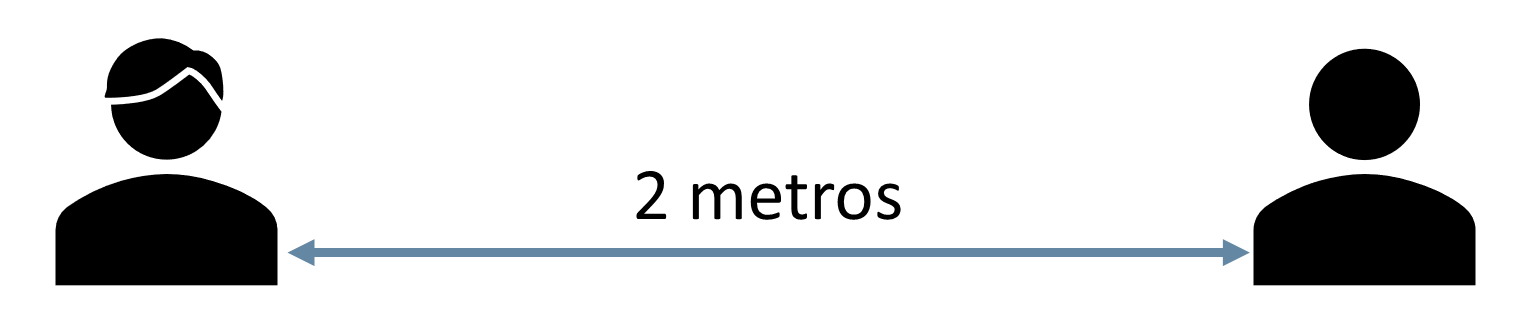
\includegraphics[scale=0.8]{Imagenes/Gravitacion_Universal_01.png}
\end{figure}
\end{frame}
\begin{frame}
\frametitle{Resolviendo el ejercicio}
\textocolor{red}{Datos:}
\begin{align*}
m_{1} &= \SI{63}{\kilo\gram} \\[0.3em]
m_{2} &= \SI{82}{\kilo\gram} \\[0.3em]
r &= \SI{2}{\meter} \\[0.3em]
G &= \SI[per-mode=fraction]{6.67d-11}{\newton\square\meter\per\square\kilo\gram}
\end{align*}
\end{frame}
\begin{frame}
\frametitle{Resolviendo el ejercicio}
\textocolor{red}{Expresión:}
\pause
\begin{align*}
F = G \, \dfrac{m_{1} \, m_{2}}{r^{2}}
\end{align*}
\end{frame}
\begin{frame}
\frametitle{Resolviendo el ejercicio}
\textocolor{red}{Sustitución:}
\pause
\begin{eqnarray*}
\begin{aligned}
F &= \dfrac{\left( \displaystyle \SI[per-mode=fraction]{6.67d-11}{\newton\square\meter\per\square\kilo\gram}\right)  (\SI{63}{\kilo\gram})(\SI{82}{\kilo\gram}) }{(\SI{2}{\meter})^{2}} = \\[0.5em] \pause
F &= \SI{8.61d-8}{\newton}
\end{aligned}
\end{eqnarray*}
\end{frame}
\begin{frame}
\frametitle{Enunciado de otro ejercicio}
Un cuerpo ($m_{1}$) de \SI{20}{\kilogram} se encuentra a \SI{5}{\meter} de otro cuerpo ($m_{2}$), entre ambos existe una fuerza de atracción de \SI{60d-11}{\newton}.
\\
\bigskip
\pause
Calcula la masa del otro cuerpo.
\begin{figure}
    \centering
    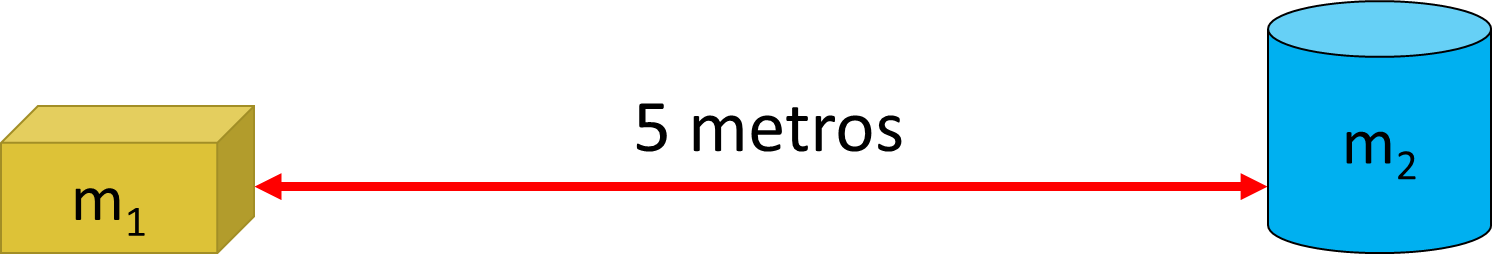
\includegraphics[scale=0.75]{Imagenes/Gravitacion_Universal_02.png}
\end{figure}
\end{frame}
\begin{frame}
\frametitle{Ejercicio para entregar 1}
La solución se debe de entregar a mano para la siguiente clase, contando $2$ punto de Evaluación Continua.
\end{frame}
\begin{frame}
\frametitle{Enunciado de otro ejercicio}
Calcula la distancia de separación entre un cuerpo de \SI{3}{\kilo\gram} y otro de \SI{8}{\kilo\gram}, si entre ambos existe una fuerza de atracción de \SI{9d-9}{\newton}
\begin{figure}
    \centering
    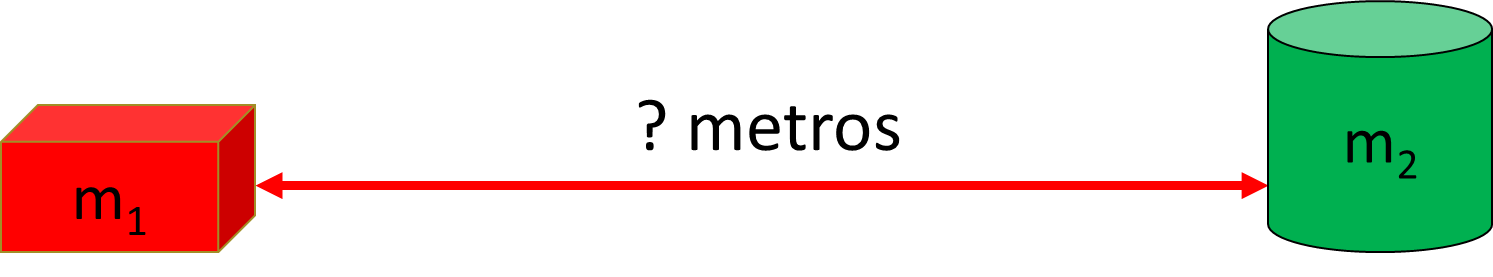
\includegraphics[scale=0.75]{Imagenes/Gravitacion_Universal_03.png}
\end{figure}
\end{frame}
\begin{frame}
\frametitle{Ejercicio para entregar 2}
La solución se debe de entregar a mano para la siguiente clase, contando $2$ punto de Evaluación Continua.
\end{frame}    

% \section{Leyes de Kepler}
% \frame[allowframebreaks]{\tableofcontents[currentsection, hideothersubsections]}
% \subsection{El trabajo de Kepler}
    
% \begin{frame}
% \frametitle{El trabajo de Kepler}
% El astrónomo alemán Johannes Kepler es conocido por sus tres leyes que describen el movimiento de los planetas en sus órbitas alrededor del Sol.
% \end{frame}
% \begin{frame}
% \frametitle{El trabajo de Kepler}
% \begin{figure}
%     \centering
%     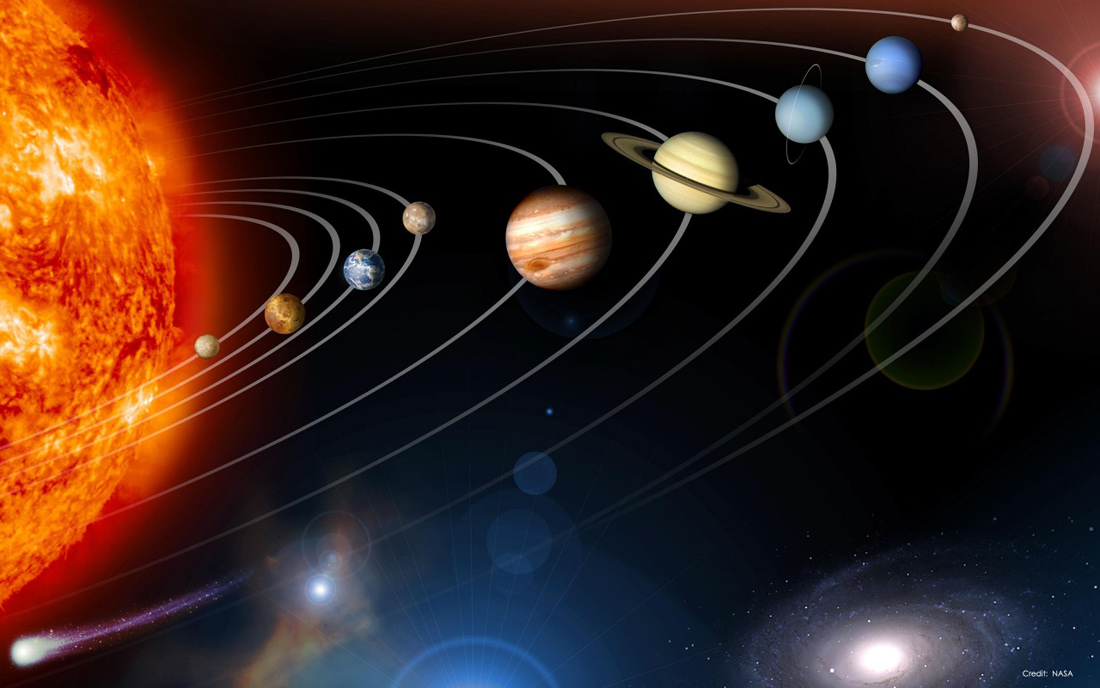
\includegraphics[scale=0.25]{Imagenes/Kepler_01.jpg}
% \end{figure}
% \end{frame}
% \begin{frame}
% \frametitle{Apoyándose con trabajos previos}
% Kepler descubrió que las \textocolor{cobalt}{trayectorias que los planetas describen alrededor del Sol eran elípticas}, \pause basándose en lo descrito por Apolonio de Pérgamo, quien desarrolló estudios sobre la elipse.
% \end{frame}

% \subsection{Primera ley}

% \begin{frame}
% \frametitle{Enunciado de la primera ley}
% Todos los planetas se desplazan alrededor del Sol siguiendo \textocolor{byzantine}{órbitas elípticas}, situando al Sol en uno de sus focos.
% \end{frame}
% \begin{frame}
% \frametitle{Enunciado de la primera ley}
% \begin{figure}
%     \centering
%     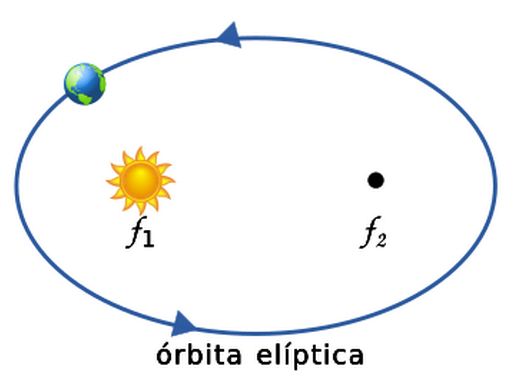
\includegraphics[scale=0.4]{Imagenes/Kepler_Leyes_01.png}
% \end{figure}
% \end{frame}
% \begin{frame}
% \frametitle{De la primera ley}
% En particular, hay dos puntos de interés en la órbita elíptica de la Tierra alrededor del Sol.
% \end{frame}
% \begin{frame}
% \frametitle{De la primera ley}
% \begin{figure}
%     \centering
%     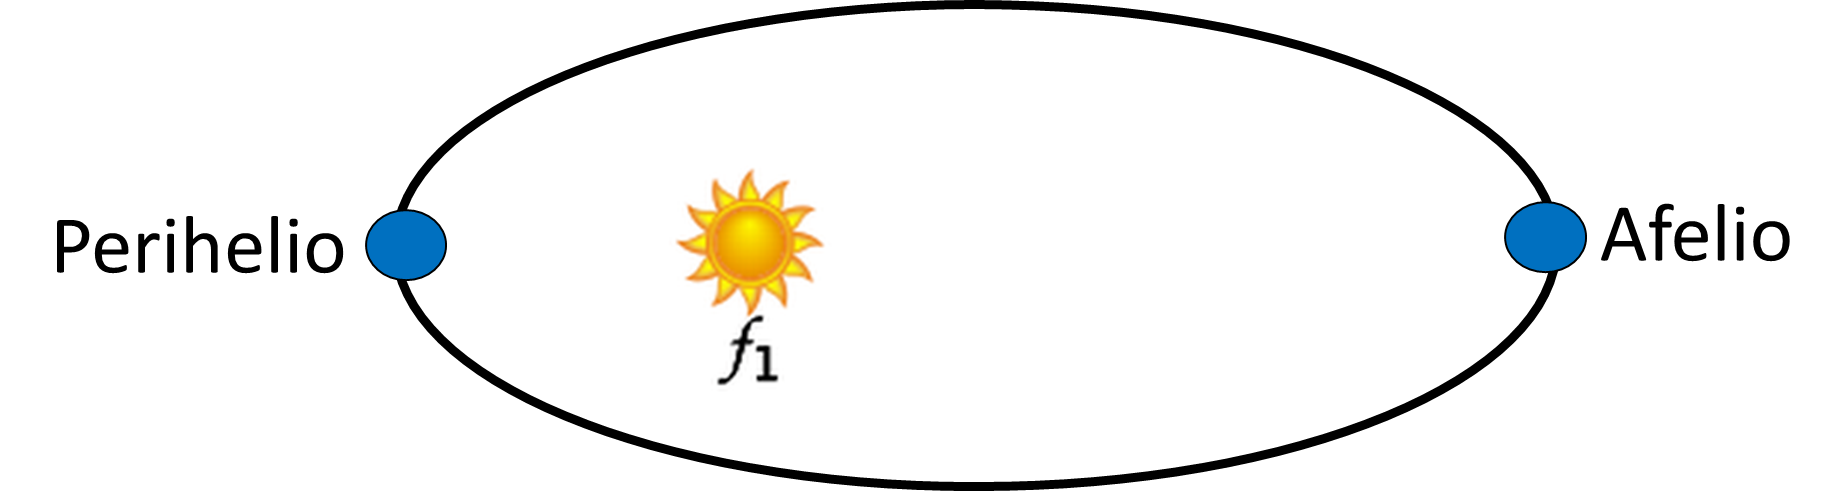
\includegraphics[scale=0.75]{Imagenes/Kepler_Leyes_01_b.png}
% \end{figure}
% \end{frame}

% \subsection{Segunda ley}

% \begin{frame}
% \frametitle{Enunciado de la segunda ley}
% La línea imaginaria que une cualquiera de los planetas con el Sol \textocolor{bulgarianrose}{barre áreas iguales en tiempos iguales}, \pause es decir, cuando el planeta está en el \textocolor{cadmiumgreen}{afelio}, su velocidad es menor que cuando está en el \textocolor{cadmiumred}{perihelio}.
% \end{frame}
% \begin{frame}
% \frametitle{Segunda ley de Kepler}
% \begin{figure}
%     \centering
%     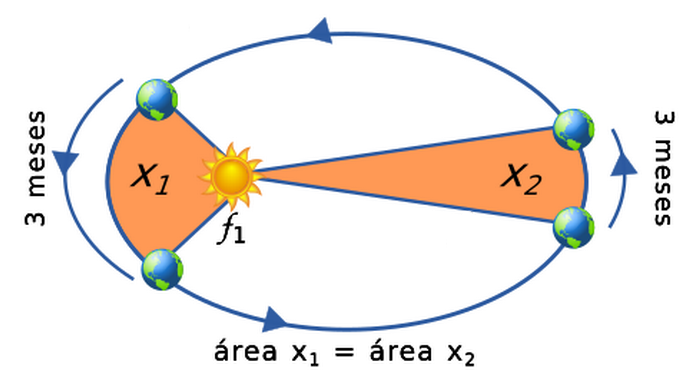
\includegraphics[scale=0.45]{Imagenes/Kepler_Leyes_02.png}
% \end{figure}
% \end{frame}
% \begin{frame}
% \frametitle{De la segunda ley}
% Kepler demostró que los planetas tienen una mayor velocidad cuando se encuentran más cercanos al Sol que cuando están más lejanos.
% \end{frame}

% \subsection{Tercera ley}


% \begin{frame}
% \frametitle{Enunciado de la tercera ley}
% El \textocolor{red}{cuadrado del período} ($T$) de cualquier planeta tiene una variación directamente proporcional con el \textocolor{cardinal}{cubo del radio de su órbita} ($r$), \pause  es decir, con el cubo de la distancia promedio que existe desde un planeta hasta el Sol.
% \end{frame}
% \begin{frame}
% \frametitle{Enunciado de la tercera ley}    
% Matemáticamente, se expresa con la fórmula:
% \pause
% \begin{align*}
% T^{2} = k \, r^{3}
% \end{align*}
% donde $k$ es una constante de proporcionalidad, que tiene el mismo valor para todos los planetas.
% \end{frame}

% \section{Trabajo en física}
% \frame[allowframebreaks]{\tableofcontents[currentsection, hideothersubsections]}
% \subsection{Definición}

% \begin{frame}
% \frametitle{El concepto de Energía}
% El concepto de \textocolor{blue-violet}{energía} es fundamental en la física y se refiere a la capacidad de un sistema para realizar trabajo.
% \end{frame}
% \begin{frame}
% \frametitle{Transformando la energía}
% La energía puede manifestarse de diferentes formas y puede ser \textocolor{red}{transformada} de una forma a otra, \pause pero la \textocolor{cobalt}{cantidad total de energía} en un sistema aislado \textocolor{cobalt}{se conserva}, de acuerdo con el principio de conservación de la energía.
% \end{frame}
% \begin{frame}
% \frametitle{Ejemplo de transformación}
% En el motor de automóvil, la energía química almacenada en el combustible se convierte parcialmente en la energía del movimiento del auto, y parcialmente en energía térmica.
% \end{frame}
% \begin{frame}
% \frametitle{Ejemplo de transformación}    
% \begin{figure}
%     \centering
%     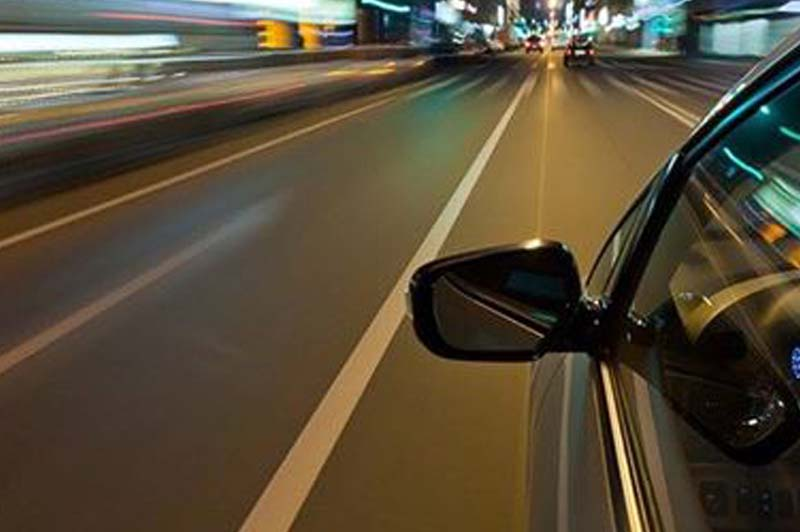
\includegraphics[scale=0.3]{Imagenes/Energia_01.jpg}
% \end{figure}
% \end{frame}
% \begin{frame}
% \frametitle{Ejemplo de transformación}    
% En un horno de microondas, la energía electromagnética obtenida de la CFE se convierte en energía térmica en el alimento caliente o cocido.
% \end{frame}
% \begin{frame}
% \frametitle{Ejemplo de transformación}    
% \begin{figure}
%     \centering
%     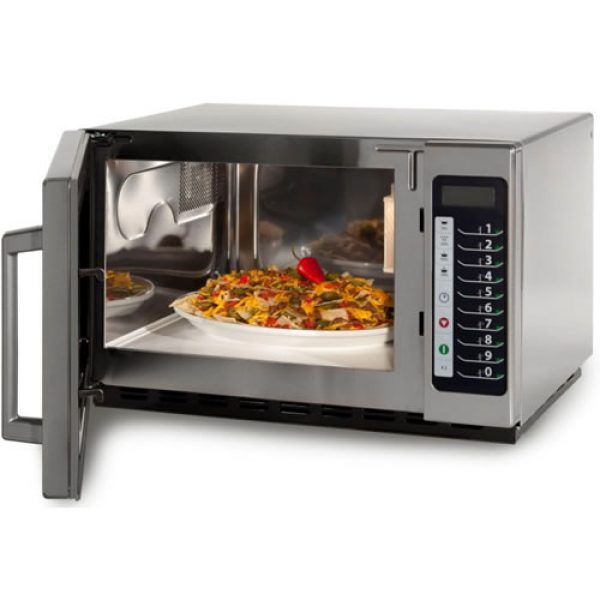
\includegraphics[scale=0.3]{Imagenes/Energia_02.jpg}
% \end{figure}
% \end{frame}

% \subsection{Conceptos clave}

% \begin{frame}
% \frametitle{El trabajo mecánico}
% El \textocolor{americanrose}{trabajo mecánico (T)} se refiere a la transferencia de energía de un objeto a otro debido a una fuerza aplicada a lo largo de una distancia.
% \end{frame}
% \begin{frame}
% \frametitle{Energía cinética}
% La \textocolor{ao(english)}{energía cinética $(E_{k})$}  se refiere a la energía asociada al movimiento de un objeto. $E_{k} = \dfrac{1}{2} m \, v^{2}$
% \begin{figure}
%     \centering
%     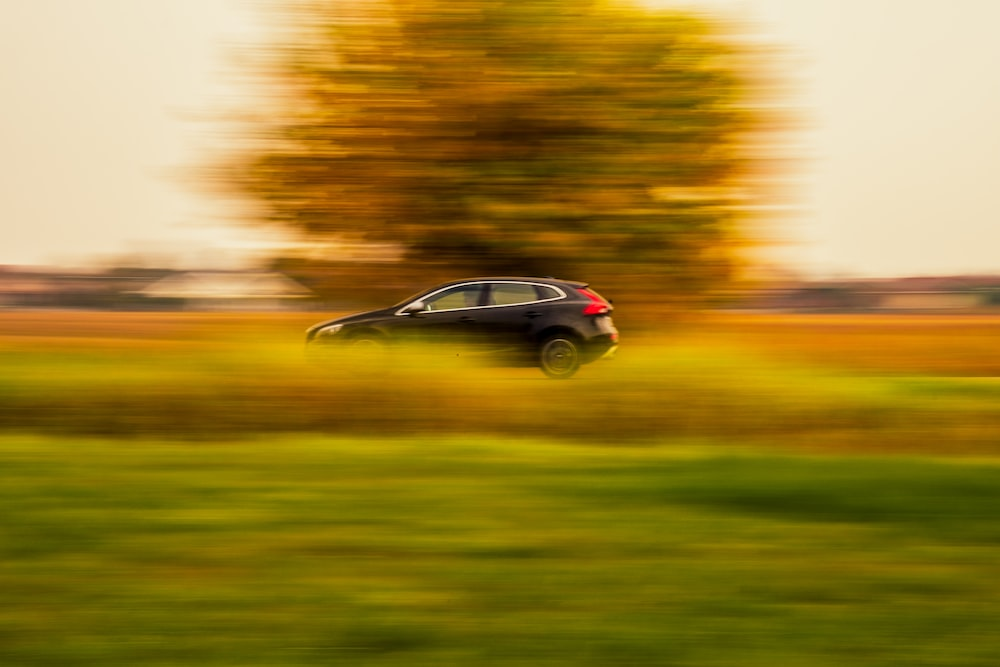
\includegraphics[scale=0.2]{Imagenes/Energia_cinetica_01.jpg}
% \end{figure}
% \end{frame}
% \begin{frame}
% \frametitle{Energía potencial}
% La \textocolor{blue(pigment)}{energía potencial $(E_{p})$} es la energía asociada con la posición o el estado de un objeto. $E_{p} = m g h$
% \begin{figure}
%     \centering
%     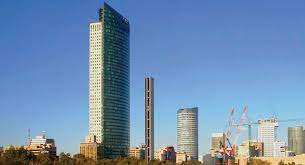
\includegraphics[scale=0.7]{Imagenes/Energia_potencial_01.jpg}
% \end{figure}
% \end{frame}
% \begin{frame}
% \frametitle{Energía mecánica}
% La \textocolor{bronze}{energía mecánica $(E_{T})$} es la suma de la \textocolor{ao(english)}{energía cinética} y la \textocolor{blue(pigment)}{energía potencial} de un objeto en un sistema. 
% \begin{align*}
% E_{t} = E_{k} + E_{p}
% \end{align*}
% \end{frame}
% \begin{frame}
% \frametitle{Energía térmica}
% La \textocolor{burntumber}{energía térmica} se refiere a la energía asociada con la temperatura de un objeto o un sistema.
% \begin{figure}
%     \centering
%     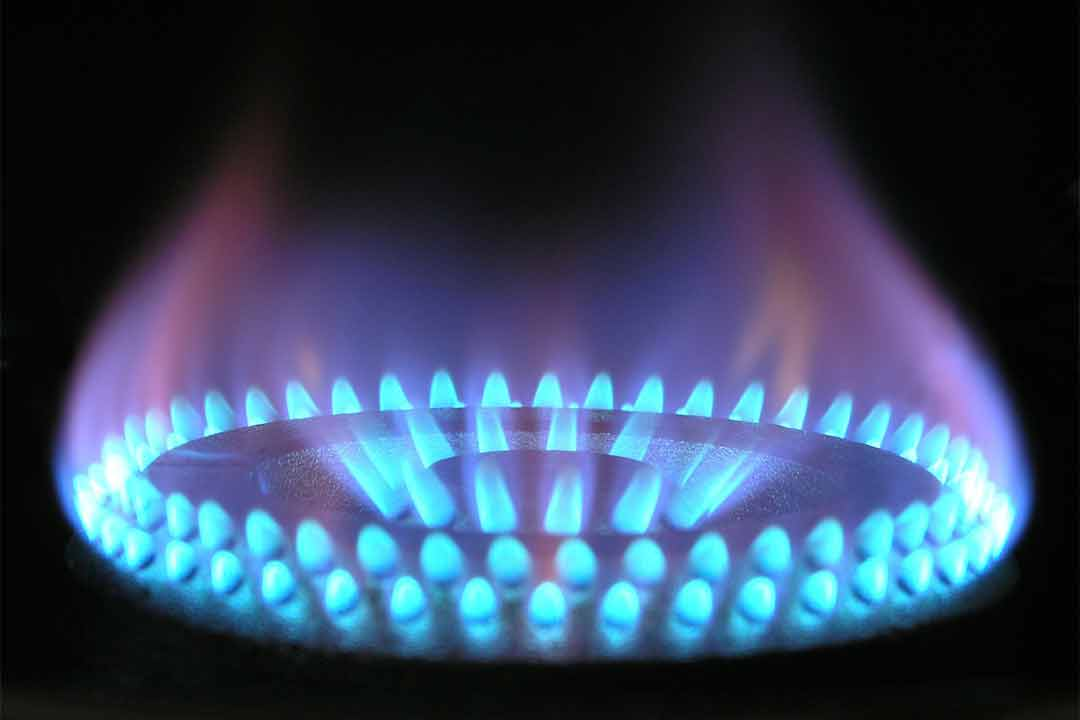
\includegraphics[scale=0.15]{Imagenes/Energia_termica_01.jpg}
% \end{figure}
% \end{frame}
% \begin{frame}
% \frametitle{Ley de conservación de la energía}
% La energía total de un sistema aislado se mantiene constante. 
% \end{frame}

% \subsection{Trabajo mecánico}

% \begin{frame}
% \frametitle{Comprendiendo el trabajo}
% Podemos pensar en trabajo mecánico, cuando vemos a una persona transportar un objeto pesado o cuando subimos las escaleras.
% \\
% \bigskip
% \pause
% Realizar un trabajo implica consumir energía.
% \end{frame}
% \begin{frame}
% \frametitle{Comprendiendo el trabajo}
% \begin{figure}
%     \centering
%     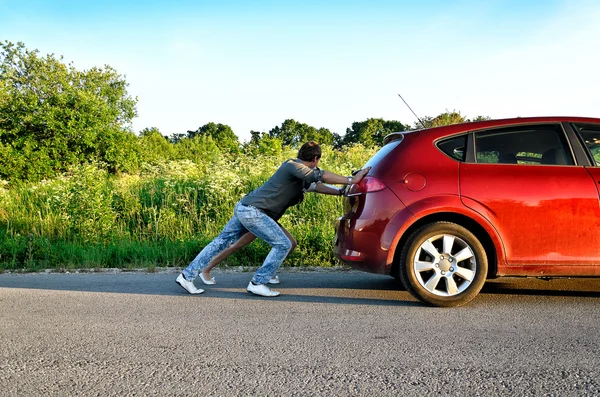
\includegraphics[scale=0.4]{Imagenes/Energia_03.png}
% \end{figure}
% \end{frame}
% \begin{frame}
% \frametitle{Factores en el trabajo}
% En todos los casos en los que se realiza un trabajo, intervienen tres factores:
% \pause
% \setbeamercolor{item projected}{bg=darkred,fg=white}
% \setbeamertemplate{enumerate items}{%
% \usebeamercolor[bg]{item projected}%
% \raisebox{1.5pt}{\colorbox{bg}{\color{fg}\footnotesize\insertenumlabel}}%
% }
% \begin{enumerate}[<+->]
% \item La aplicación de una fuerza.
% \item El desplazamiento.
% \item Una componente a lo largo del desplazamiento.
% \end{enumerate}
% \end{frame}
% \begin{frame}
% \frametitle{Consideraciones para la definición}
% Si se considera que la fuerza es constante y el movimiento es en línea recta y en la dirección de la fuerza.
% \end{frame}
% \begin{frame}
% \frametitle{Definición del trabajo mecánico}
% Entonces el \textocolor{blue}{trabajo mecánico} que realiza la fuerza aplicada sobre un objeto se define como el producto de la fuerza por distancia que recorre el objeto.
% \end{frame}
% \begin{frame}
% \frametitle{Expresión para el trabajo}
% La expresión es:
% \begin{align*}
% T = F \cdot d \hspace{0.5cm} \rightarrow \hspace{0.5cm} \left[ J \quad (\text{Joule}) \right]
% \end{align*}
% \pause
% Donde:
% \setbeamercolor{item projected}{bg=deepcarmine,fg=white}
% \setbeamertemplate{enumerate items}{%
% \usebeamercolor[bg]{item projected}%
% \raisebox{1.5pt}{\colorbox{bg}{\color{fg}\footnotesize\insertenumlabel}}%
% }
% \begin{enumerate}[<+->]
% \item $F$ es la fuerza (en Newtons)
% \item $d$ es la distancia (en metros)
% \item $T$ es el trabajo medido en Joules (Newton por metro)
% \end{enumerate}
% \end{frame}
% \begin{frame}
% \frametitle{Triángulo del Trabajo}
% \begin{figure}
%     \centering
%     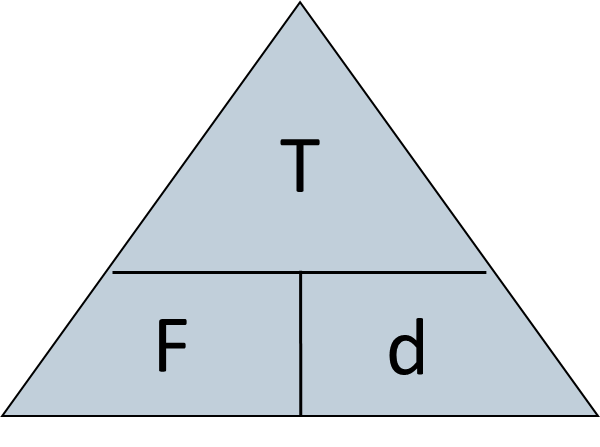
\includegraphics[scale=1]{Imagenes/Triangulo_Trabajo.png}
% \end{figure}
% \end{frame}
% \begin{frame}
% \frametitle{Enunciado del Ejercicio}
% Un barco remolcador ejerce una fuerza constante de \SI{5000}{\newton} sobre un barco que se mueve con  velocidad constante a través del mar.
% \\
% \bigskip
% \pause
% ¿Cuánto trabajo hace el remolcador sobre el barco en una distancia de \SI{3}{\kilo\meter}?
% \end{frame}
% \begin{frame}
% \frametitle{Resolviendo el ejercicio}
% \textocolor{red}{Datos:}
% \pause
% \begin{align*}
% F &= \SI{5000}{\newton} \\[0.5em]
% d &= \SI{3}{\kilo\meter} = \SI{3000}{\meter}
% \end{align*}
% \end{frame}
% \begin{frame}
% \frametitle{Resolviendo el ejercicio}
% \textocolor{red}{Expresión:}
% \begin{figure}
%     \centering
%     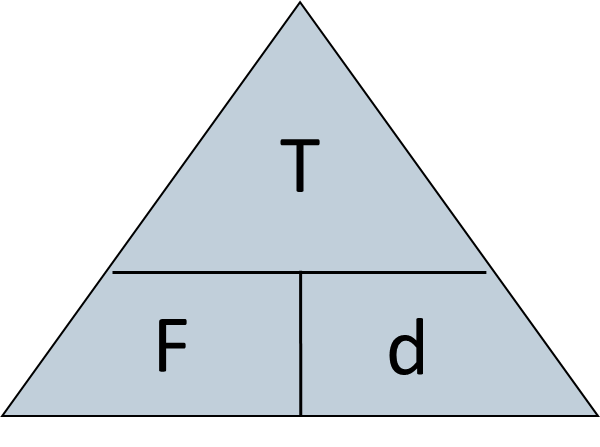
\includegraphics[scale=0.75]{Imagenes/Triangulo_Trabajo.png}
% \end{figure}
% \pause
% \begin{align*}
% T = F \cdot d
% \end{align*}
% \end{frame}
% \begin{frame}
% \frametitle{Resolviendo el ejercicio}
% \textocolor{red}{Sustitución:}
% \begin{eqnarray*}
% \begin{aligned}
% T &= (\SI{5d3}{\newton})(\SI{3d3}{\meter}) = \\[0.5em] \pause 
% T &= \SI{15d6}{\newton\meter} = \\[0.5em] \pause 
% T &= \SI{15d6}{\joule} 
% \end{aligned}
% \end{eqnarray*}
% \end{frame}
% \begin{frame}
% \frametitle{Enunciado de otro ejercicio}
% Un hombre carga el paquete que recibió a la puerta de su casa, la caja indica el contenido de \SI{55}{\kilo\gram}, recorre \SI{90}{\centi\meter} y lo apoya en la mesa.
% \\
% \bigskip
% \pause
% ¿Cuánto trabajo realiza el hombre?
% \end{frame}
% \begin{frame}
% \frametitle{Resolviendo el ejercicio}
% \textocolor{red}{Datos:}
% \pause
% \begin{align*}
% m &= \SI{55}{\kilo\gram} \\[0.5em]
% d &= \SI{90}{\centi\meter} = \SI{0.9}{\meter} \\[0.5em]
% F &= \, ? \\[0.5em]
% T &= \, ?
% \end{align*}
% \end{frame}
% \begin{frame}
% \frametitle{Resolviendo el ejercicio}
% \textocolor{red}{Expresiones:}
% \begin{align*}
% F &= m \, g \\[0.5em]
% T &= F \cdot d
% \end{align*}
% \end{frame}
% \begin{frame}
% \frametitle{Resolviendo el ejercicio}
% \textocolor{red}{Sustituciones:}
% \begin{eqnarray*}
% \begin{aligned}
% F &= (\SI{55}{\kilo\gram})(\SI{9.81}{\meter\per\square\second}) = \pause \SI{539.55}{\newton} \\[0.5em] \pause
% T &= (\SI{539.55}{\newton})(\SI{0.9}{\meter}) = \pause \SI{485.89}{\joule}
% \end{aligned}
% \end{eqnarray*}
% \end{frame}
% % \begin{frame}
% % \frametitle{Enunciado de otro ejercicio}
% % Para arrancar un auto de \SI{800}{\kilo\gram} de transmisión estándar \enquote{en segunda}, se necesita como mínimo recorrer \SI{5}{\meter} de distancia. \pause Si entre varios amigos realizaron un trabajo de \SI{3.5d4}{\joule} al empujarlo:
% % \setbeamercolor{item projected}{bg=electricgreen,fg=black}
% % \setbeamertemplate{enumerate items}{%
% % \usebeamercolor[bg]{item projected}%
% % \raisebox{1.5pt}{\colorbox{bg}{\color{fg}\footnotesize\insertenumlabel}}%
% % }
% % \begin{enumerate}[<+->]
% % \item ¿Lograron que el auto arrancara?
% % \item ¿Qué trabajo se requiere exactamente para que el auto arranque?
% % \end{enumerate}
% % \end{frame}

% \section{Energía}
% \frame[allowframebreaks]{\tableofcontents[currentsection, hideothersubsections]}
% \subsection{Definición}

% \begin{frame}
% \frametitle{La energía en física}
% La \textocolor{cobalt}{energía} es la capacidad para desarrollar un trabajo.
% \\
% \bigskip
% \pause
% Su unidad son los Joules (J), equivale a un newton por metro (\unit{\newton\meter}).
% \end{frame}
% \begin{frame}
% \frametitle{Energía constante}
% La energía que existe en el Universo \textocolor{byzantine}{es constante},\pause es decir, su cantidad total no aumenta ni disminuye.
% \end{frame}
% \begin{frame}
% \frametitle{Ley de conservación de la energía}
% La energía existente en el Universo no se crea ni se destruye, sólo se transforma.
% \end{frame}

% \subsection{Energía cinética}

% \begin{frame}
% \frametitle{Definición}
% Es la energía que genera un cuerpo al estar en movimiento.
% \\
% \bigskip
% \pause
% \begin{align*}
% E_{k} = \dfrac{1}{2} m \, v^{2}
% \end{align*}
% \end{frame}
% \begin{frame}
% \frametitle{Enunciado del ejercicio}
% Calcula la energía cinética de un vehículo de \SI{1000}{\kilo\gram} de masa que circula a una velocidad de \SI{120}{\kilo\meter\per\hour}.
% \end{frame}
% \begin{frame}
% \frametitle{Resolviendo el ejercicio}
% \textocolor{red}{Datos:} \pause m = \SI{1000}{\kilo\gram}, \pause v = \SI{120}{\kilo\meter\per\hour}
% \\
% \bigskip
% \pause
% \textocolor{red}{Expresión:} $E_{k} = \dfrac{1}{2} m \, v^{2}$
% \end{frame}
% \begin{frame}
% \frametitle{Resolviendo el ejercicio}
% \textocolor{red}{Sustitución:}
% \pause
% \begin{eqnarray*}
% \begin{aligned}
% E_{k} &= \dfrac{1}{2} (\SI{1000}{\kilo\gram}) \left( \SI[per-mode=fraction]{120}{\kilo\meter\per\hour} \right)^{2} = \\[0.5em] \pause
% E_{k} &= \dfrac{1}{2} (\SI{1000}{\kilo\gram}) \left( \SI[per-mode=fraction]{33.33}{\meter\per\second} \right)^{2} = \\[0.5em] \pause
% E_{k} &= \SI{555444.45}{\joule}
% \end{aligned}
% \end{eqnarray*}
% \end{frame}
% \begin{frame}
% \frametitle{Enunciado de otro ejercicio}
% Calcula la velocidad a la que va trotando una persona de \SI{65}{\kilo\gram} que adquiera una energía cinética de \SI{700}{\joule}.
% \end{frame}
% \begin{frame}
% \frametitle{Resolviendo el ejercicio}
% \textocolor{red}{Datos:} \pause m = \SI{65}{\kilo\gram}, \pause $E_{k} = \SI{700}{\joule}$
% \\
% \bigskip
% \pause
% \textocolor{red}{Expresión:}
% \begin{eqnarray*}
% \begin{aligned}
% E_{k} &= \dfrac{1}{2} m \, v^{2} \\[0.5em] \pause
% v = \sqrt{\dfrac{2 \, E_{k}}{m}}
% \end{aligned}
% \end{eqnarray*}
% \end{frame}
% \begin{frame}
% \frametitle{Resolviendo el ejercicio}
% \textocolor{red}{Sustitución:}
% \pause
% \begin{eqnarray*}
% \begin{aligned}
% v &= \sqrt{\dfrac{2 \, \SI{700}{\joule}}{\SI{65}{\kilo\gram}}} = \pause \sqrt{\dfrac{2 \, \SI{700}{\newton\meter}}{\SI{65}{\kilo\gram}}} = \\[0.5em]\pause 
% v &= \sqrt{\dfrac{2 \, \SI[per-mode=fraction]{700}{\kilo\gram\square\meter\per\square\second}}{\SI{65}{\kilo\gram}}} = \pause \sqrt{\SI[per-mode=fraction]{21.53}{\square\meter\per\square\second}} = \\[0.5em] \pause
% v &= \SI[per-mode=fraction]{4.64}{\meter\per\second}
% \end{aligned}
% \end{eqnarray*}
% \end{frame}    

% \subsection{Energía potencial}

% \begin{frame}
% \frametitle{Definición de la energía potencial}
% Es la energía que tiene un cuerpo por su posición, \textocolor{cadmiumgreen}{con respecto de la horizontal o altura}, es también llamada energía gravitatoria.
% \end{frame}
% \begin{frame}
% \frametitle{Expresión para la energía potencial}
% Para obtener la energía potencial $E_{p}$, se ocupa la siguiente expresión:
% \pause
% \begin{align*}
% E_{p} = m \, g \, h
% \end{align*}
% \end{frame}
% \begin{frame}
% \frametitle{Enunciado del ejercicio}
% Calcula la energía potencial que posee un libro de \SI{500}{\gram} de masa que está colocado sobre una mesa de \SI{80}{\centi\meter} de altura.
% \end{frame}
% \begin{frame}
% \frametitle{Resolviendo el ejercicio}
% \textocolor{red}{Datos:} \pause m = \SI{50}{\gram}, \pause $h = \SI{80}{\centi\meter}$
% \\
% \bigskip
% \pause
% \textocolor{red}{Expresión:}
% \begin{eqnarray*}
% \begin{aligned}
% E_{p} &= m \, g \, h
% \end{aligned}
% \end{eqnarray*}
% \end{frame}
% \begin{frame}
% \frametitle{Resolviendo el ejercicio}
% \textocolor{red}{Sustitución:}
% \pause
% \begin{eqnarray*}
% \begin{aligned}
% E_{p} &= (\SI{0.5}{\kilo\gram}) \left( \SI{9.81}{\meter\per\square\second} \right) (\SI{0.8}{\meter}) = \\[0.5em] \pause
% E_{p} &= \SI{3.92}{\joule}
% \end{aligned}
% \end{eqnarray*}
% \end{frame}
% \begin{frame}
% \frametitle{Ejercicio por resolver}
% ¿En qué piso de un estacionamiento se encuentra un auto de \SI{840}{\kilo\gram} para que se energía potencial sea de \SI{39600}{\joule}?
% \\
% \bigskip
% Cada piso mide \SI{2.4}{\meter}
% \end{frame}
% \begin{frame}
% \frametitle{Ejercicio por resolver}
% Calcula la masa de un objeto que se levanta hasta una altura de \SI{12}{\meter} que adquiere una energía potencial de \SI{2120}{\joule}.
% \end{frame}
% \begin{frame}
% \frametitle{Ejercicio por resolver}
% Un balón de \SI{600}{\gram} se patea hacia  arriba con una velocidad de \SI{35}{\meter\per\second}. \pause Calcula:
% \pause
% \setbeamercolor{item projected}{bg=bananayellow,fg=black}
% \setbeamertemplate{enumerate items}{%
% \usebeamercolor[bg]{item projected}%
% \raisebox{1.5pt}{\colorbox{bg}{\color{fg}\footnotesize\insertenumlabel}}%
% }
% \begin{enumerate}[<+->]
% \item El valor inicial de las energías cinética y potencial.
% \seti
% \end{enumerate}
% \end{frame}
% \begin{frame}
% \frametitle{Ejercicio por resolver}
% \setbeamercolor{item projected}{bg=bananayellow,fg=black}
% \setbeamertemplate{enumerate items}{%
% \usebeamercolor[bg]{item projected}%
% \raisebox{1.5pt}{\colorbox{bg}{\color{fg}\footnotesize\insertenumlabel}}%
% }
% \begin{enumerate}[<+->]    
% \conti
% \item La energía cinética y potencial a los \SI{20}{\meter} de altura.
% \item Demuestra que la energía mecánica se conserva.
% \end{enumerate}
% \end{frame}
    

\end{document}